% Modelo de Tese/Dissertação para UNIFEI
\documentclass[
% opções da classe memoir
12pt,
oneside,
a4paper,
oldfontcommands,
% opções do pacote babel
english,			% idioma adicional para hifenização
brazil				% o último idioma é o principal do documento
]{abntex2} 

% configurações (pacotes, comandos)
\input{Configuracoes/config.tex}
% informações (título, autor, instituição, banca examinadora, etc.)
%%%%%%%%%%%%%%%%%%%%%%%%%%%%%%%%%%%%%%%%%%%%%%%%%%%%%%%%%%%%%%%%%%%%%%%%%
%
% ALTERAR AS INFORMAÇÕES DESSE BLOCO
%
%%%%%%%%%%%%%%%%%%%%%%%%%%%%%%%%%%%%%%%%%%%%%%%%%%%%%%%%%%%%%%%%%%%%%%%%%
%%%%%%%%%%%%%%%%%%%%%%%%%%%%%%%%%%%%%%%%%%%%%%%%%%%%%%%%%%%%%%%%%%%%%%%%%

% IMPORTANTE: Inserir aqui o tipo do trabalho (mestrado ou doutorado)
%\def \tipo{doutorado}
\def \tipo{mestrado}

% Informações de dados para CAPA e FOLHA DE ROSTO
%\titulo{rqt\_mrta: Uma Interface Gráfica de Usuário baseada em ROS para configuração e supervisão de Arquiteturas de Alocação de Tarefas em Sistema Multirrobô}
%\titulo{rqt\_mrta: Uma interface gráfica para configuração e supervisão de Arquiteturas de Alocação de Tarefa em Sistema Multirrobô no ROS}
%\titulo{rqt\_mrta: Uma GUI para configuração e supervisão de Arquiteturas MRTA no ROS}
%\titulo{rqt\_mrta: Uma aplicação para configuração e supervisão de Arquiteturas MRTA no ROS}
\titulo{rqt\_mrta: Um Pacote ROS para Configuração e Supervisão de Arquiteturas MRTA}
\autor{Adriano Henrique Rossette Leite}
\local{Itajubá}
\data{\today}
\orientador{Prof. Dr. Guilherme Sousa Bastos}
%\coorientador{Prof. Dr. Coorientador}
\instituicao{Universidade Federal de Itajubá}
\def \programaLinhaUm{Programa de Pós-Graduação em}
\def \programaLinhaDois{Engenharia Elétrica}
\def \programa{\programaLinhaUm \space \programaLinhaDois}
\def \areaconcentracao{Automação e Sistemas Elétricos Industriais}

% Data de aprovação
\def \diadeaprovacao{15}
\def \mesdeaprovacao{Dezembro}
\def \anodeaprovacao{2017}

% Banca examinadora - Professores convidados
\def \professorConvidadoUm{Prof. Dr. Edson Prestes}
\def \professorConvidadoDois{Prof. Dr. Laércio Augusto Baldochi Júnior}
%\def \professorConvidadoTres{Prof. Dr. Guilherme Sousa Bastos}

%%%%%%%%%%%%%%%%%%%%%%%%%%%%%%%%%%%%%%%%%%%%%%%%%%%%%%%%%%%%%%%%%%%%%%%%%
%%%%%%%%%%%%%%%%%%%%%%%%%%%%%%%%%%%%%%%%%%%%%%%%%%%%%%%%%%%%%%%%%%%%%%%%%
%%%%%%%%%%%%%%%%%%%%%%%%%%%%%%%%%%%%%%%%%%%%%%%%%%%%%%%%%%%%%%%%%%%%%%%%%
%%%%%%%%%%%%%%%%%%%%%%%%%%%%%%%%%%%%%%%%%%%%%%%%%%%%%%%%%%%%%%%%%%%%%%%%%

\ifthenelse{\equal{\tipo}{mestrado}}{
    \def \tipoTrabalhoUm{Dissertação}
    \def \tipoTrabalhoDois{Mestrado}
    \def \titulacao{Mestre}
}{
    
    \ifthenelse{\equal{\tipo}{doutorado}}{
        \def \tipoTrabalhoUm{Tese}
        \def \tipoTrabalhoDois{Doutorado}
        \def \titulacao{Doutor}
    }{
        \def \tipoTrabalhoUm{Undefined}
        \def \tipoTrabalhoDois{Undefined}
        \def \titulacao{Undefined}
    }
}

\tipotrabalho{\tipoTrabalhoUm \space (\tipoTrabalhoDois)}

% O preambulo deve conter o tipo do trabalho, o objetivo, o nome da instituição e a área de concentração 
\preambulo{\tipoTrabalhoUm \space submetida ao \programa \space como parte dos requisitos para obtenção do Título de \titulacao \space em Ciências em \programaLinhaDois.}

% frase utilizada na folha de aprovação
\def  \aprovacao{\large \tipoTrabalhoUm \space aprovada por banca examinadora em \diadeaprovacao \space de \mesdeaprovacao \space de \anodeaprovacao, conferindo ao autor o título de \textbf {\titulacao \space em Ciências em \programaLinhaDois.}}

% Banca examinadora
\def \bancaexaminadora{\professorConvidadoUm 
    \\ \professorConvidadoDois
    %\\ \professorConvidadoTres
}

% Início do documento
\begin{document}

% Elementos pré-textuais
% Capa
\input{1_Pre_Texto/capa.tex}
% Folha de Rosto
\input{1_Pre_Texto/folhaderosto.tex}
% Folha de Aprovação 1
\input{1_Pre_Texto/folhadeaprovacao1.tex}
% Ficha Catalográfica
\input{1_Pre_Texto/fichacatalografica.tex}
% Folha de Aprovação 2
\input{1_Pre_Texto/folhadeaprovacao2.tex}
% Agradecimentos
\begin{agradecimentos}
À Deus ...

À meus amigos e familiares ...

Ao meu orientador ...

À banca examinadora, ...

Aos amigos e colegas do LRO, ...

À Capes pelo apoio financeiro durante estes 2 anos. 

À Fapemig pelo financiamento do projeto de pesquisa TEC-APQ-00666-12, o qual possibilitou a compra do robô utilizado neste trabalho~(Pioneer-3DX).
\end{agradecimentos}
\newpage
% Epígrafe
\begin{epigrafe}
    \vspace*{\fill}
	\begin{flushright}
	\textit{``I may never find all the answers.\\
	         I may never understand why.\\
	         I may never prove what I know to be true.\\
	         But I know that I still have to try.''\\
		(Dream Theater)}
	\end{flushright}
\end{epigrafe}
\newpage
% Resumo
\newpage
% resumo em português
\begin{resumo}
    Este trabalho apresenta o desenvolvimento do pacote baseado em ROS \textit{rqt\_mrta}, o qual fornece um \textit{plugin} de interface gráfica de usuário para a parametrização amigável de arquiteturas para a resolução de problemas de alocação de tarefa em sistema multirrobô. Além disso, em tempo de execução, o \textit{plugin} dispõe elementos gráficos para a supervisão e monitoramento da arquitetura e do sistema multirrobô. Utilizando uma aplicação de testes com a arquitetura ALLIANCE, pode-se constatar que o pacote reduziu a complexidade da tarefa de parametrização de arquiteturas de alocação de tarefa
    \vspace{\onelineskip}
    
    \noindent
    \textbf{Palavras-chaves}: ALLIANCE. Alocação de Tarefa. Arquitetura. ROS. Sistema Multirrobô. 
\end{resumo}
\newpage
% Resumo em inglês - abstract
\begin{resumo}[Abstract]
    \begin{otherlanguage*}{english}
        This work presents the \textit{rqt\_mrta}, an ROS-based project that provides a Graphical User Interface (GUI) plugin for configuring multirobot task allocation (MRTA) architectures. Moreover, it arranges graphical elements for system supervision and monitoration them during runtime. A generic approach of the ALLIANCE architecture is developed in order to test and validate this graphical tool by creating a multirobot patrol application. The results shows that the usage of the \textit{rqt\_mrta} plugin facilitates the parametrization of MRTA architectures.
        
        \vspace{\onelineskip}
        
        \noindent 
        \textbf{Key-words}: ALLIANCE. Architecture. Multirobot System. ROS. Task Allocation. 
    \end{otherlanguage*}
\end{resumo}
\newpage
% Lista de ilustrações
\input{1_Pre_Texto/listailustracoes.tex}
% Lista de tabelas
\input{1_Pre_Texto/listatabelas.tex}
% Lista de abreviaturas e siglas
% inserir lista de abreviaturas e siglas
\renewcommand{\nomname}{\listadesiglasname}
\pdfbookmark[0]{\nomname}{las}
\cleardoublepage
% inserir em ordem alfabética
\begin{siglas}
    \item[ABNT] Associação Brasileira de Normas Técnicas
    \item[API] \textit{Application Programming Interface}
    \item[CBR] Competição Brasileira de Robótica
    \item[CNP] \textit{Contract Net Protocol}
    \item[GPU] \textit{Graphics Processing Unit}
    \item[GUI] \textit{Graphical User Interface}
    \item[LRO] Laboratório de Robótica
    \item[MAS] \textit{Multi-Agent System}
    \item[MRS] \textit{Multi-Robot System}
    \item[MRTA] \textit{Multi-Robot Task Allocation}
    \item[MVC] \textit{Model-View-Controller}
    \item[OAP] \textit{Optimal Assignment Problem}
    \item[P3DX] \textit{Adept MobileRobots Pioneer 3 DX}
    \item[ROS] \textit{Robot Operating System}
    \item[UI] \textit{User Interface}
    \item[UML] \textit{Unified Modeling Language}
    \item[UNIFEI] Universidade Federal de Itajubá
    \item[XML] \textit{Extensible Markup Language}
    \item[YAML] \textit{YAML Ain't Markup Language}
\end{siglas}
% Lista de símbolos
% inserir lista de símbolos
\renewcommand{\nomname}{\listadesimbolosname}
\pdfbookmark[0]{\nomname}{las}
\cleardoublepage
% inserir em ordem alfabética
\begin{simbolos} 	
    \item[$n$] Número inteiro
    \item[$t$] Tempo
    \item[$T$] Período
\end{simbolos}
% Sumário
\input{1_Pre_Texto/sumario.tex}

% Elementos textuais
\textual
% Introdução
\chapter[Introdução]{Introdução} \label{cap:introducao}

    \section{Motivação} \label{sec:motivacao}
        Aplicações de robótica onde vários robôs interagem entre si e também com o ambiente em que estão inseridos são chamadas de sistemas multirrobô, do inglês \textit{Multi-robot systems} (MRS). Um sistema multirrobô possui diversas vantagens sobre sistemas com apenas um robô. Entre elas se encontram o ganho de flexibilidade, a simplificação de tarefas complexas e o aumento da eficiência no uso de recursos, de desempenho do sistema como um todo e da robustez através de redundâncias \cite{ref:cao1997cooperative, ref:dudek1996taxonomy, ref:zlot2002multi}. Entretanto, aplicações dessa natureza demandam arquiteturas complexas para o controle da coordenação dos robôs envolvidos e, intrinsecamente, possuem problema de escalabilidade nos processos computacionais e na rede de comunicação. 
        
        Um dos problemas mais desafiadores em aplicações de vários robôs é denominado \textit{alocação de tarefa} (MRTA, acrônimo para \textit{Multi-Robot Task Allocation}), que busca atribuir a execução de um conjunto de tarefas para um grupo de robôs sujeitos à limitações de forma que o desempenho geral do sistema seja otimizado. Esse tipo de problema pode ser resolvido por arquiteturas que se baseiam em modelos de organização que podem ser encontrados no cotidiano. Suas premissas limitam a abrangência de problemas que podem ser resolvidos pela a arquitetura. Com isso, há uma grande quantidade de arquiteturas formuladas. E com o intuito de classificá-las, \citeonline{ref:gerkey2004taxonomy} sugeriu uma taxonomia independente do domínio para a classificação de problemas MRTA a partir da análise de várias delas \cite{ref:parker1998alliance, ref:gerkey2002murdoch, ref:botelho1999m+, ref:werger2000ble, ref:frank2005kuhn, ref:stentz1999fpo, ref:chaimowicz2002dra}. 
        
        Com o advento do ROS (do inglês \textit{Robot Operating System}) \cite{ref:quigley2009ros}, vários sistemas inteligentes puderam ser reutilizados em diversas aplicações de robótica, tais como: localização \cite{ref:li2017kld-samcl}, navegação robótica, gerenciamento de largura de banda \cite{ref:julio2015dynamic}, planejamento e escalonamento de ações e tarefas \cite{ref:fox2003pddl2, ref:manne1960job}, algoritmos de inteligência artificial \cite{ref:adrianohrl2015fuzzy, ref:watkins1992qlearning}, entre outros. Sendo um \textit{middleware} dedicado para aplicações robóticas, ele possibilitou a integração de trabalhos desenvolvidos por equipes distintas de pesquisa em robótica, pois ele simplifica o desenvolvimento de processos e dá suporte à comunicação e interoperabilidade deles. Desta forma, pesquisadores de robótica podem ater-se ao desenvolvimento de projetos dentro da sua especialização, necessitando apenas configurar os demais pacotes para a execução da aplicação. Problemas que anteriormente possuíam difícil solução em termos de \textit{software}, foram simplificados a partir da modularidade proporcionada pelo ROS.
        
        Apesar da vasta existência de arquiteturas de alocação de tarefa para sistemas multirrobôs, houveram poucas tentativas de aproximação genérica delas em projetos baseados em ROS. \textcolor{red}{Isto é, mediante a pesquisa realizada na literatura e no repositório do ROS, não foram encontrados projetos baseados em ROS que se aproximam de uma arquitetura MRTA configurável para qualquer problema MRTA que satisfaça suas premissas. \citeonline{ref:reis2015alliance} mostraram as facilidades que o ROS oferece na implementação da arquitetura ALLIANCE, proposta por \citeonline{ref:parker1998alliance}. Contudo, essa aproximação atende apenas o problema aplicado nesse trabalho. Já em \textit{ auction\_methods\_stack}\footnote{\url{https://github.com/joaoquintas/auction_methods_stack}}, ainda que não possui documentação alguma, está contido um grupo de pacotes que foi desenvolvido em uma versão antiga do ROS e nunca mais foi atualizado.}
        
        Com isso, verifica-se a necessidade de ferramentas que facilitem a utilização de arquiteturas de alocação de tarefa em sistemas multirrobô para o \textit{framework} ROS para incentivar o desenvolvimento de aproximações genéricas dessas arquiteturas.
    
    \section{Objetivos} \label{sec:objetivos}
        Esse trabalho propõe desenvolver um pacote ROS, denominado \textit{rqt\_mrta}, que facilite a utilização de arquiteturas de alocação de tarefa no ROS para sistemas multirrobô. Esse pacote fornece uma interface gráfica que foi desenvolvida com o intuito de disponibilizar serviços para dois tipos de clientes: (1) desenvolvedor e (2) usuário de arquitetura MRTA. Seus serviços são:
        
        \begin{itemize}
            \item Cadastro de novas arquiteturas no ROS para seu uso na solução de problemas de alocação de tarefa em sistemas multirrobô;
            \item Criação de novos projetos contendo a definição de um problema de alocação de tarefa;
            \item Configuração da arquitetura escolhida para resolver o problema MRTA;
            \item Armazenamento dos dados de configuração no projeto criado;
            \item Monitoramento da comunicação dos robôs do sistema no ROS em tempo de execução;
            \item Monitoramento das atividades dos robôs no sistema em tempo de execução.
        \end{itemize}
        
        Além disso, será apresentado neste trabalho uma aproximação genérica da arquitetura Alliance, a qual foi desenvolvida em um pacote ROS chamado \textit{alliance}.
        
    \section{Contribuições} \label{sec:contribuicoes}
        A partir da elaboração deste trabalho, os seguintes pacotes baseados em ROS foram obtidos e disponibilizados para a comunidade ROS:
        
        \begin{itemize}
            \item \textbf{\textit{rqt\_mrta}}\footnote{\url{http://wiki.ros.org/rqt_mrta}}: uma interface gráfica usuário que facilita a utilização de arquiteturas que resolvem o problema de alocação de tarefa em um sistema multirrobô.
            \item \textbf{\textit{alliance}}\footnote{\url{http://wiki.ros.org/alliance}}: uma aproximação genérica da arquitetura Alliance.
            \item \textbf{\textit{alliance\_msgs}}\footnote{\url{http://wiki.ros.org/alliance_msgs}}: contém definição das mensagens utilizadas na comunicação entre os robôs na arquitetura Alliance pelo pacote \textit{alliance}.
            \item \textbf{\textit{rqt\_alliance}}\footnote{\url{http://wiki.ros.org/rqt_alliance}}: uma interface gráfica de usuário que monitora as variáveis de motivação dos robôs em um sistema que utiliza o pacote \textit{alliance} para a alocação de tarefas.
        \end{itemize}
    
    \section{Estrutura do Trabalho} \label{sec:estrutura}
        No capítulo \ref{cap:revisao}, ... 
        Prosseguindo para o capítulo \ref{cap:desenvolvimento}, ...
        A seguir, ..., no capítulo \ref{cap:resultados}.
        Por fim, o capítulo \ref{cap:conclusao} ...
% Capítulos
\chapter[Revisão teórica]{Revisão teórica} \label{cap:revisao}
    Colocar texto aqui 
    
    \section{Sistema Multirrobô} \label{sec:mrs}
        Colocar texto aqui
    
        \subsection{Taxonomias} \label{subsec:taxonomias_mrs}
    
    \section{Alocação de Tarefa em Sistema Multirrobô} \label{sec:mrta}
        Um dos problemas mais desafiadores em aplicações multirrobô leva o nome \textit{alocação de tarefa}, na língua inglesa, \textit{Multi-Robot Task Allocation}(MRTA). Problemas dessa natureza buscam como solução atribuir otimamente um conjunto de robôs para um conjunto de tarefas de maneira que o desempenho geral de um sistema sujeito a um conjunto de limitações seja otimizado.
        
        \textcolor{red}{falar sobre o conteúdo desta seção}
        
        
        \subsection{Definição Formal} \label{subsec:mrta_formal}
            \citeonline{ref:zlot2006auction} define o problema de alocação de tarefa em um sistema multirrobô conforme abaixo.
            
            \begin{definicao} \label{def:mrta}
                (\textit{Alocação de Tarefa em um Sistema Multirrobô})
                Sejam dados um conjunto $T$, um conjunto $R$ e uma função de custo para cada subconjunto de robots $r \in R$ que especifique o custo de performance para cada subconjunto de tarefas, $c_r : 2^T \to \mathbb{R}_+\cup\{\infty\}$: procure a alocação $A^* \in R^T$ que minimiza a função objetivo global $C : R^T \to \mathbb{R}_+\cup\{\infty\}$.
            \end{definicao}
        
            Note que para que um algoritmo consiga encontrar uma solução ótima para este problema, é necessário levar em consideração todo o espaço de alocação $R^T$, cujo tamanho aumenta exponencialmente em função do número de tarefas e robôs no sistema. 
            
            %Muitas arquiteturas simplificam este problema possa ter uma solução viável em tempo real.
            
            
    
        \subsection{Taxonomia} \label{subsec:taxonomia_mrta}
            \citeonline{ref:gerkey2004taxonomy} sugeriram uma taxonomia de três eixos independente do domínio para a classificação de problemas de alocação de tarefas em sistemas multirrobôs. 
            
            O primeiro eixo determina o \textit{tipo dos robôs} que compõem o problema. Os tipos de robôs possíveis são: \textit{ST} (acrônimo para \textit{Single-Task}) ou \textit{MT} (acrônimo para \textit{Multi-Task}). Problemas que envolvem robôs que só podem executar uma tarefa por vez são compostos por robôs do tipo \textit{ST}. Entretanto, se houver pelo menos um robô capaz de executar mais de uma tarefa simultaneamente, então esse problema é composto por robôs do tipo \textit{MT}. 
            
            O segundo eixo da taxonomia determina o \textit{tipo das tarefas} que compõem o problema. Nesse caso, são possíveis os tipos: \textit{ST} (acrônimo para \textit{Single-Robot}) ou \textit{MR} (acrônimo para \textit{Multi-Robot}). Problemas cujo tipo das tarefas é \textit{SR}, diz-se que todas as tarefas envolvidas só podem ser executadas por um robô. Porém, quando o tipo das tarefas envolvidas é \textit{MR}, diz-se que existe tarefas que podem ser executadas por mais de um robô.
            
            O terceiro eixo, por sua vez, determina o \textit{tipo da alocação} do problema, o qual pode assumir os valores: \textit{IA} (acrônimo para \textit{Instantaneous Assignment}) ou \textit{TA} (acrônimo para \textit{Time-extended Assignment}). O primeiro caso, \textit{IA}, diz repeito à problemas MRTA onde as alocações das tarefas para os robôs são realizadas instantaneamente, sem levar em consideração o estado futuro do sistema. Por outro lado, em problemas cujo tipo de alocação é \textit{TA}, além de conhecido o estado atual de cada rôbo e do ambiente, também é conhecido o conjunto de tarefas que precisarão ser alocadas no futuro. Neste último caso, diversas tarefas são alocadas para um robô, o qual deve executar cada alocação conforme seu agendamento. De acordo com \cite{ref:bastos2008utility}, quando o tipo de alocação do problema MRTA é \textit{IA}, o número de robôs é superior ao número de tarefas alocadas e quando \textit{TA}, o oposto acontece. Isso se deve ao fato de que, em problemas MRTA cujo tipo de alocação é \textit{IA}, o número de robôs no sistema é capaz de suprir a taxa de tarefas a serem atribuídas, de modo que é muito provável que haverão robôs ociosos no sistema; enquanto, naqueles cujo tipo de alocação é \textit{TA}, o número de robôs que compõem o sistema não é suficiente para atender a taxa de tarefas a serem alocadas no sistema.
            
            \begin{figure}[htb]
                \centering
                % Graphic for TeX using PGF
% Title: ../figures/taxonomia_mrta.dia
% Creator: Dia v0.97.2
% CreationDate: Tue Oct 17 17:33:09 2017
% For: adrianohrl
% \usepackage{tikz}
% The following commands are not supported in PSTricks at present
% We define them conditionally, so when they are implemented,
% this pgf file will use them.
\ifx\du\undefined
  \newlength{\du}
\fi
\setlength{\du}{15\unitlength}
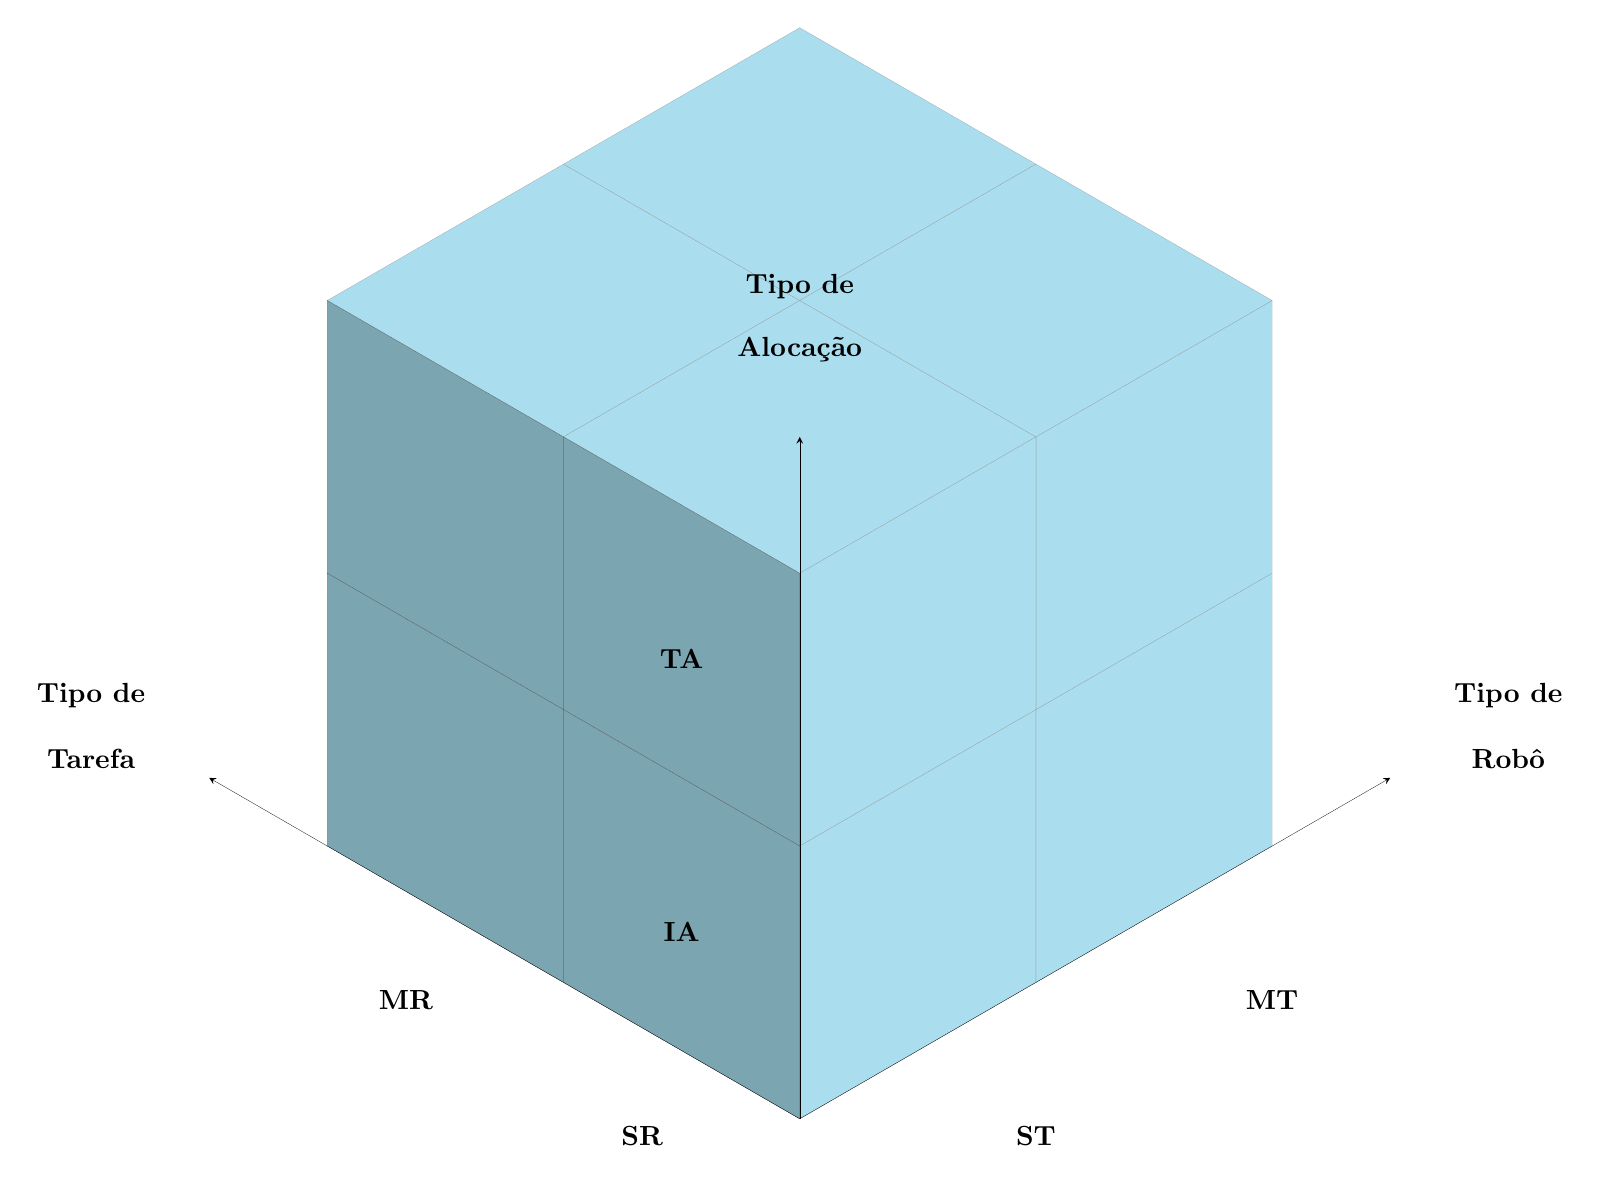
\begin{tikzpicture}
\pgftransformxscale{1.000000}
\pgftransformyscale{-1.000000}
\definecolor{dialinecolor}{rgb}{0.000000, 0.000000, 0.000000}
\pgfsetstrokecolor{dialinecolor}
\definecolor{dialinecolor}{rgb}{1.000000, 1.000000, 1.000000}
\pgfsetfillcolor{dialinecolor}
\pgfsetlinewidth{0.050000\du}
\pgfsetdash{}{0pt}
\pgfsetdash{}{0pt}
\pgfsetmiterjoin
\pgfsetbuttcap
\definecolor{dialinecolor}{rgb}{0.666667, 0.870588, 0.937255}
\pgfsetfillcolor{dialinecolor}
\fill (-5.500000\du,-10.392300\du)--(-2.500000\du,-8.660250\du)--(0.500000\du,-10.392300\du)--(-2.500000\du,-12.124400\du)--cycle;
\definecolor{dialinecolor}{rgb}{0.556863, 0.556863, 0.556863}
\pgfsetstrokecolor{dialinecolor}
\draw (-5.500000\du,-10.392300\du)--(-2.500000\du,-8.660250\du)--(0.500000\du,-10.392300\du)--(-2.500000\du,-12.124400\du)--cycle;
\pgfsetlinewidth{0.050000\du}
\pgfsetdash{}{0pt}
\pgfsetdash{}{0pt}
\pgfsetmiterjoin
\pgfsetbuttcap
\definecolor{dialinecolor}{rgb}{0.666667, 0.870588, 0.937255}
\pgfsetfillcolor{dialinecolor}
\fill (-2.500000\du,-12.124400\du)--(0.500000\du,-10.392300\du)--(3.500000\du,-12.124400\du)--(0.500000\du,-13.856400\du)--cycle;
\definecolor{dialinecolor}{rgb}{0.556863, 0.556863, 0.556863}
\pgfsetstrokecolor{dialinecolor}
\draw (-2.500000\du,-12.124400\du)--(0.500000\du,-10.392300\du)--(3.500000\du,-12.124400\du)--(0.500000\du,-13.856400\du)--cycle;
\pgfsetlinewidth{0.050000\du}
\pgfsetdash{}{0pt}
\pgfsetdash{}{0pt}
\pgfsetmiterjoin
\pgfsetbuttcap
\definecolor{dialinecolor}{rgb}{0.666667, 0.870588, 0.937255}
\pgfsetfillcolor{dialinecolor}
\fill (3.500000\du,-8.660250\du)--(3.500000\du,-5.196150\du)--(6.500000\du,-6.928200\du)--(6.500000\du,-10.392300\du)--cycle;
\definecolor{dialinecolor}{rgb}{0.556863, 0.556863, 0.556863}
\pgfsetstrokecolor{dialinecolor}
\draw (3.500000\du,-8.660250\du)--(3.500000\du,-5.196150\du)--(6.500000\du,-6.928200\du)--(6.500000\du,-10.392300\du)--cycle;
\pgfsetlinewidth{0.050000\du}
\pgfsetdash{}{0pt}
\pgfsetdash{}{0pt}
\pgfsetmiterjoin
\pgfsetbuttcap
\definecolor{dialinecolor}{rgb}{0.666667, 0.870588, 0.937255}
\pgfsetfillcolor{dialinecolor}
\fill (-2.500000\du,-8.660250\du)--(0.500000\du,-6.928200\du)--(3.500000\du,-8.660250\du)--(0.500000\du,-10.392300\du)--cycle;
\definecolor{dialinecolor}{rgb}{0.556863, 0.556863, 0.556863}
\pgfsetstrokecolor{dialinecolor}
\draw (-2.500000\du,-8.660250\du)--(0.500000\du,-6.928200\du)--(3.500000\du,-8.660250\du)--(0.500000\du,-10.392300\du)--cycle;
\pgfsetlinewidth{0.050000\du}
\pgfsetdash{}{0pt}
\pgfsetdash{}{0pt}
\pgfsetmiterjoin
\pgfsetbuttcap
\definecolor{dialinecolor}{rgb}{0.666667, 0.870588, 0.937255}
\pgfsetfillcolor{dialinecolor}
\fill (0.500000\du,-10.392300\du)--(3.500000\du,-8.660250\du)--(6.500000\du,-10.392300\du)--(3.500000\du,-12.124400\du)--cycle;
\definecolor{dialinecolor}{rgb}{0.556863, 0.556863, 0.556863}
\pgfsetstrokecolor{dialinecolor}
\draw (0.500000\du,-10.392300\du)--(3.500000\du,-8.660250\du)--(6.500000\du,-10.392300\du)--(3.500000\du,-12.124400\du)--cycle;
\pgfsetlinewidth{0.050000\du}
\pgfsetdash{}{0pt}
\pgfsetdash{}{0pt}
\pgfsetmiterjoin
\pgfsetbuttcap
\definecolor{dialinecolor}{rgb}{0.666667, 0.870588, 0.937255}
\pgfsetfillcolor{dialinecolor}
\fill (0.500000\du,-6.928200\du)--(0.500000\du,-3.464100\du)--(3.500000\du,-5.196150\du)--(3.500000\du,-8.660250\du)--cycle;
\definecolor{dialinecolor}{rgb}{0.556863, 0.556863, 0.556863}
\pgfsetstrokecolor{dialinecolor}
\draw (0.500000\du,-6.928200\du)--(0.500000\du,-3.464100\du)--(3.500000\du,-5.196150\du)--(3.500000\du,-8.660250\du)--cycle;
\pgfsetlinewidth{0.050000\du}
\pgfsetdash{}{0pt}
\pgfsetdash{}{0pt}
\pgfsetmiterjoin
\pgfsetbuttcap
\definecolor{dialinecolor}{rgb}{0.666667, 0.870588, 0.937255}
\pgfsetfillcolor{dialinecolor}
\fill (0.500000\du,-3.464100\du)--(0.500000\du,0.000000\du)--(3.500000\du,-1.732050\du)--(3.500000\du,-5.196150\du)--cycle;
\definecolor{dialinecolor}{rgb}{0.556863, 0.556863, 0.556863}
\pgfsetstrokecolor{dialinecolor}
\draw (0.500000\du,-3.464100\du)--(0.500000\du,0.000000\du)--(3.500000\du,-1.732050\du)--(3.500000\du,-5.196150\du)--cycle;
\pgfsetlinewidth{0.050000\du}
\pgfsetdash{}{0pt}
\pgfsetdash{}{0pt}
\pgfsetmiterjoin
\pgfsetbuttcap
\definecolor{dialinecolor}{rgb}{0.666667, 0.870588, 0.937255}
\pgfsetfillcolor{dialinecolor}
\fill (3.500000\du,-5.196150\du)--(3.500000\du,-1.732050\du)--(6.500000\du,-3.464100\du)--(6.500000\du,-6.928200\du)--cycle;
\definecolor{dialinecolor}{rgb}{0.556863, 0.556863, 0.556863}
\pgfsetstrokecolor{dialinecolor}
\draw (3.500000\du,-5.196150\du)--(3.500000\du,-1.732050\du)--(6.500000\du,-3.464100\du)--(6.500000\du,-6.928200\du)--cycle;
\pgfsetlinewidth{0.050000\du}
\pgfsetdash{}{0pt}
\pgfsetdash{}{0pt}
\pgfsetmiterjoin
\pgfsetbuttcap
\definecolor{dialinecolor}{rgb}{0.486275, 0.647059, 0.698039}
\pgfsetfillcolor{dialinecolor}
\fill (-2.500000\du,-8.660250\du)--(-2.500000\du,-5.196150\du)--(-5.500000\du,-6.928200\du)--(-5.500000\du,-10.392300\du)--cycle;
\definecolor{dialinecolor}{rgb}{0.290196, 0.290196, 0.290196}
\pgfsetstrokecolor{dialinecolor}
\draw (-2.500000\du,-8.660250\du)--(-2.500000\du,-5.196150\du)--(-5.500000\du,-6.928200\du)--(-5.500000\du,-10.392300\du)--cycle;
\pgfsetlinewidth{0.050000\du}
\pgfsetdash{}{0pt}
\pgfsetdash{}{0pt}
\pgfsetmiterjoin
\pgfsetbuttcap
\definecolor{dialinecolor}{rgb}{0.486275, 0.647059, 0.698039}
\pgfsetfillcolor{dialinecolor}
\fill (0.500000\du,-6.928200\du)--(0.500000\du,-3.464100\du)--(-2.500000\du,-5.196150\du)--(-2.500000\du,-8.660250\du)--cycle;
\definecolor{dialinecolor}{rgb}{0.290196, 0.290196, 0.290196}
\pgfsetstrokecolor{dialinecolor}
\draw (0.500000\du,-6.928200\du)--(0.500000\du,-3.464100\du)--(-2.500000\du,-5.196150\du)--(-2.500000\du,-8.660250\du)--cycle;
\pgfsetlinewidth{0.050000\du}
\pgfsetdash{}{0pt}
\pgfsetdash{}{0pt}
\pgfsetmiterjoin
\pgfsetbuttcap
\definecolor{dialinecolor}{rgb}{0.486275, 0.647059, 0.698039}
\pgfsetfillcolor{dialinecolor}
\fill (-2.500000\du,-5.196150\du)--(-2.500000\du,-1.732050\du)--(-5.500000\du,-3.464100\du)--(-5.500000\du,-6.928200\du)--cycle;
\definecolor{dialinecolor}{rgb}{0.290196, 0.290196, 0.290196}
\pgfsetstrokecolor{dialinecolor}
\draw (-2.500000\du,-5.196150\du)--(-2.500000\du,-1.732050\du)--(-5.500000\du,-3.464100\du)--(-5.500000\du,-6.928200\du)--cycle;
\pgfsetlinewidth{0.050000\du}
\pgfsetdash{}{0pt}
\pgfsetdash{}{0pt}
\pgfsetmiterjoin
\pgfsetbuttcap
\definecolor{dialinecolor}{rgb}{0.486275, 0.647059, 0.698039}
\pgfsetfillcolor{dialinecolor}
\fill (0.500000\du,-3.464100\du)--(0.500000\du,0.000000\du)--(-2.500000\du,-1.732050\du)--(-2.500000\du,-5.196150\du)--cycle;
\definecolor{dialinecolor}{rgb}{0.290196, 0.290196, 0.290196}
\pgfsetstrokecolor{dialinecolor}
\draw (0.500000\du,-3.464100\du)--(0.500000\du,0.000000\du)--(-2.500000\du,-1.732050\du)--(-2.500000\du,-5.196150\du)--cycle;
% setfont left to latex
\definecolor{dialinecolor}{rgb}{0.000000, 0.000000, 0.000000}
\pgfsetstrokecolor{dialinecolor}
\node at (-8.500000\du,-5.374900\du){\textbf{Tipo de}};
% setfont left to latex
\definecolor{dialinecolor}{rgb}{0.000000, 0.000000, 0.000000}
\pgfsetstrokecolor{dialinecolor}
\node at (-8.500000\du,-4.574900\du){\textbf{Tarefa}};
% setfont left to latex
\definecolor{dialinecolor}{rgb}{0.000000, 0.000000, 0.000000}
\pgfsetstrokecolor{dialinecolor}
\node at (0.500000\du,-10.571050\du){\textbf{Tipo de}};
% setfont left to latex
\definecolor{dialinecolor}{rgb}{0.000000, 0.000000, 0.000000}
\pgfsetstrokecolor{dialinecolor}
\node at (0.500000\du,-9.771050\du){\textbf{Alocação}};
% setfont left to latex
\definecolor{dialinecolor}{rgb}{0.000000, 0.000000, 0.000000}
\pgfsetstrokecolor{dialinecolor}
\node at (9.500000\du,-5.374900\du){\textbf{Tipo de}};
% setfont left to latex
\definecolor{dialinecolor}{rgb}{0.000000, 0.000000, 0.000000}
\pgfsetstrokecolor{dialinecolor}
\node at (9.500000\du,-4.574900\du){\textbf{Robô}};
\pgfsetlinewidth{0.100000\du}
\pgfsetdash{}{0pt}
\pgfsetdash{}{0pt}
\pgfsetbuttcap
{
\definecolor{dialinecolor}{rgb}{0.000000, 0.000000, 0.000000}
\pgfsetfillcolor{dialinecolor}
% was here!!!
\pgfsetarrowsstart{stealth}
\definecolor{dialinecolor}{rgb}{0.000000, 0.000000, 0.000000}
\pgfsetstrokecolor{dialinecolor}
\draw (8.000000\du,-4.330130\du)--(0.500000\du,0.000000\du);
}
\pgfsetlinewidth{0.100000\du}
\pgfsetdash{}{0pt}
\pgfsetdash{}{0pt}
\pgfsetbuttcap
{
\definecolor{dialinecolor}{rgb}{0.000000, 0.000000, 0.000000}
\pgfsetfillcolor{dialinecolor}
% was here!!!
\pgfsetarrowsstart{stealth}
\definecolor{dialinecolor}{rgb}{0.000000, 0.000000, 0.000000}
\pgfsetstrokecolor{dialinecolor}
\draw (-7.000000\du,-4.330130\du)--(0.500000\du,0.000000\du);
}
% setfont left to latex
\definecolor{dialinecolor}{rgb}{0.000000, 0.000000, 0.000000}
\pgfsetstrokecolor{dialinecolor}
\node at (-4.500000\du,-1.510800\du){\textbf{MR}};
% setfont left to latex
\definecolor{dialinecolor}{rgb}{0.000000, 0.000000, 0.000000}
\pgfsetstrokecolor{dialinecolor}
\node at (-1.500000\du,0.221250\du){\textbf{SR}};
% setfont left to latex
\definecolor{dialinecolor}{rgb}{0.000000, 0.000000, 0.000000}
\pgfsetstrokecolor{dialinecolor}
\node at (3.500000\du,0.221250\du){\textbf{ST}};
% setfont left to latex
\definecolor{dialinecolor}{rgb}{0.000000, 0.000000, 0.000000}
\pgfsetstrokecolor{dialinecolor}
\node at (6.500000\du,-1.510800\du){\textbf{MT}};
% setfont left to latex
\definecolor{dialinecolor}{rgb}{0.000000, 0.000000, 0.000000}
\pgfsetstrokecolor{dialinecolor}
\node at (-1.000000\du,-5.840930\du){\textbf{TA}};
% setfont left to latex
\definecolor{dialinecolor}{rgb}{0.000000, 0.000000, 0.000000}
\pgfsetstrokecolor{dialinecolor}
\node at (-1.000000\du,-2.376830\du){\textbf{IA}};
\pgfsetlinewidth{0.100000\du}
\pgfsetdash{}{0pt}
\pgfsetdash{}{0pt}
\pgfsetbuttcap
{
\definecolor{dialinecolor}{rgb}{0.000000, 0.000000, 0.000000}
\pgfsetfillcolor{dialinecolor}
% was here!!!
\pgfsetarrowsstart{stealth}
\definecolor{dialinecolor}{rgb}{0.000000, 0.000000, 0.000000}
\pgfsetstrokecolor{dialinecolor}
\draw (0.500000\du,-8.660250\du)--(0.500000\du,0.000000\du);
}
\end{tikzpicture}

                \caption[Representação visual da taxonomia de três eixos]{Representação visual da taxonomia de três eixos sugerida por \citeonline{ref:gerkey2004taxonomy}.} \label{fig:taxomia_mrta}
            \end{figure}
            
            É visto na Figura \ref{fig:taxomia_mrta} uma representação gráfica da taxonomia de \cite{ref:gerkey2004taxonomy} para a classificação de problemas MRTA (\textit{Multi-Robot Task Allocation}), onde pode-se notar que existem oito classes de problemas MRTA bem definidos.
            
        \subsubsection{Arquitetura MRTA} \label{subsec:arquiteturas_mrta}
            Possue a função de solucionar o problema de alocação de tarefas em um dado sistema multirrobô.
            
            Basicamente existem duas formas de implementação de uma arquitetura iterativas e instantâneas. As aproximações iterativas apresentam uma dinâmica progressiva para que ocorra um alocação, enquanto as arquiteturas que esperam uma resposta instantânea dos robôs do sistema ...
        
            \subsection{Arquiteturas baseadas em Comportamento} \label{subsec:arch_comportamento}
            
            \begin{itemize}
                \item \textbf{ALLIANCE}: \cite{ref:parker1998alliance};
                \item \textbf{L-ALLIANCE}: \cite{ref:parker1996lalliance};
                
            \end{itemize}
            
            \subsection{Arquiteturas baseadas em Mercado} \label{subsec:arch_mercado}
    
            \begin{itemize}
                \item \textbf{Murdoch}: \cite{ref:gerkey2002murdoch};
                \item \textbf{M+}: \cite{ref:botelho1999m+};
                
            \end{itemize}
                
    \section{ROS - Robot Operating System} \label{sec:ros}
        Acrônimo para \textit{Robot Operating System} \cite{ref:quigley2009ros}, o ROS é um \textit{framework} para robótica que tem incentivado a comunidade de pesquisadores desta área do conhecimento a trabalhar conjuntamente desde seu lançamento. Ao observar o grande avanço desta ferramenta de comunicação, muitos fabricantes de manipuladores industriais iniciaram a investir em pesquisas para integrar seus robôs com o ROS. 
        
        Uma lacuna que antes existia na nova geração de aplicações robóticas foi preenchida com o lançamento do ROS. Como um fornecedor de serviços de \textit{middleware}, ele (1) simplifica o desenvolvimento de processos, (2) suporta comunicação e interoperabilidade, (3) oferece e facilita serviços frequentemente utilizados em robótica e, ainda, oferece (4) utilização eficiente dos seus recursos disponíveis, (5) abstrações heterogênicas e (6) descoberta e configuração automática de recursos \cite{ref:quigley2009ros}. No intuito de cobrir todas exigências de um \textit{middleware}, ROS 2.0 tenta dar suporte à sistemas embarcados e dispositivos de baixo recurso.
    
        No ROS, projetos atômicos são chamados \textit{pacotes} e podem ser desenvolvido em diversas linguagens de programação. Isso mostra que o ROS é flexível, pois seus usuários podem tirar proveito das vantagens que cada linguagem suportada tem, sejam elas eficiência em tempo de execução, confiabilidade, recursos, síntaxe, semântica, suporte ou documentação existente. Atualmente, as linguagens de programação suportadas são C++, Python e Lisp. As linguagens Java e Lua ainda estão em fase de desenvolvimento.
        
        Projetos de robótica possuem rotinas que poderia ser reutilizadas em outros projetos. Por esta razão, ROS é também modular, pois pacotes configuráveis existentes podem ser combinados para realizar uma aplicação especifica de robótica. Várias bibliotecas externas já foram adaptadas para serem usadas no ROS: aruco\footnote{\url{http://wiki.ros.org/ar_sys}}, gmapping\footnote{\url{http://wiki.ros.org/gmapping}}, interfaces de programação para aplicações de robôs\footnote{\url{http://wiki.ros.org/Robots}}, sensores\footnote{\url{http://wiki.ros.org/Sensors}} e simuladores\footnote{\url{http://wiki.ros.org/gazebo}}, planejadores\footnote{\url{http://kcl-planning.github.io/ROSPlan/}}, reconhecimento de voz\footnote{\url{http://wiki.ros.org/Sensors\#Audio_.2BAC8_Speech_Recognition}}, entre outros. Isso evidencia que os usuários de ROS podem focar no desenvolvimento de pesquisa de sua área e contribuir da melhor forma com essa comunidade.
        
        Enfim, ROS disponibiliza diversas ferramentas para auxiliar no desenvolvimento de projetos e, também, verificar o funcionamento de aplicação. Suas ferramentas típicas são: \textit{get} e \textit{set} de parâmetros de configuração, vizualização da topologia de conexão \textit{peer-to-peer}, medição de utilização de banda, gráficos dos dados de mensagem e outras mais. É altamente recomendado o uso dessas ferramentas para garantir a estabilidade e confiança dos pacotes desenvolvidos, que normalmente têm alta complexidade.
        
        Esta seção apresenta conceitos básicos para entender o funcionamento desta \textit{framework}. Em seguida, são expostas as regras de nomenclatura dos recursos do ROS. E, então, é brevemente dado suporte sobre a construção de aplicações gráficas integradas com o ROS.
        
        \subsection{Conceitos Básicos} \label{subsec:ros_conceitos}
            Sua concepção foi fundada sobre conceitos divididos em três níveis: (1) Sistema de Arquivos do ROS, (2) Grafo de Computação do ROS e (3) Comunidade do ROS. A seguir será explicado cada um desses níveis, cada um com seu respectivo conjunto de conceitos. Além disso, também serão detalhados os dois tipos de nomes definidos no ROS: nomes de recursos de pacote e nomes de recursos de grafo.
            
            \subsubsection{Sistema de Arquivos do ROS} \label{subsubsec:ros_arquivos}
                Os conceitos envolvidos no nível do \textit{Sistema de Arquivos do ROS} se referem aos arquivos armazenados em disco. São eles:
                
                \begin{itemize}
                    \item \textbf{Pacotes}: em inglês \textit{Packages}, é uma forma atômica de organização de criação e lançamento de \textit{software} no ROS. Um pacote contém definições de processos (nós), de dependência de bibliotecas, de tipos de mensagens, ações e serviços, de estruturas de dados e, por fim, de configuração. 
                    
                    \item \textbf{Meta-Pacotes}: em inglês \textit{Metapackages}, é um tipo especial de pacote que tem por objetivo agrupar pacotes relacionados.
                    
                    \item \textbf{Manifestos de Pacote}: em inglês \textit{Package Manifests}, arquivo nomeado \textit{package.xml} contido na raíz de cada pacote. Seu papel é fornecer meta-informações sobre seu pacote: nome, versão, descrição, informações de licença, dependências, entre outras. 
                    
                    \item \textbf{Tipos de Mensagem}: em inglês \textit{Message Types}, arquivos de extensão \textit{.msg}, localizados dentro da pasta \textit{msg} de um dado pacote. Seu conteúdo define a estrutura de dados de uma mensagem que poderá ser enviado pelo ROS.
                    
                    \item \textbf{Tipos de Serviço}: em inglês \textit{Service Types}, arquivos de extensão \textit{.srv}, localizados dentro da pasta \textit{srv} de um dado pacote. Seu conteúdo define a estrutura de dados das mensagens de requisito e resposta de um serviço, as quais poderão ser enviadas pelo ROS.
                \end{itemize}
            
            \subsubsection{Grafo de Computação do ROS} \label{subsubsec:ros_grafo}
                O \textit{Grafo de Computação do ROS} é uma rede ponto-a-ponto de processos que processam dados conjuntamente. Os conceitos presentes neste nível são:
                
                \begin{itemize}
                    \item \textbf{Nós}: em inglês \textit{Nodes}, são processos computacionais que são executados para desempenhar o controle de atuadores, realizar leitura e filtragem de sinais sensoriais ou implementar algoritmos avançados de planejamento e tomada de decisão. É desejável que os nós sejam desenvolvidos da forma mais genérica possível, para sua reutilização em outros projetos. Cada linguagem de programação suportada encapsula as funcionalidades do ROS em uma biblioteca. Para a escrita de um nó na linguagem C++, é utilizada a biblioteca do pacote \textit{roscpp}\footnote{\url{http://wiki.ros.org/roscpp}} e, para escrever um nó em Python, é utilizada a biblioteca contida no pacote \textit{rospy}\footnote{\url{http://wiki.ros.org/rospy}};
                    
                    \item \textbf{Nó Mestre}: em inglês \textit{Master}, fornece cadastro e pesquisa de nome no Grafo de Computação do ROS, ou seja, este nó é responsável por garantir a comunicação entre os nós. Sem a sua execução, não existe comunicação entre os nós.
                    
                    \item \textbf{Servidor de Parâmetros}: em inglês \textit{Parameter Server}, parte do Nó Mestre que centraliza a consulta e o armazenamento de dados indexados por uma cadeia de caracteres.
                    
                    \item \textbf{Mensagens}: em inglês \textit{Messages}, a comunicação entre os nós no ROS consiste no transporte de mensagens, as quais são estruturas de dados que possuem campos tipados. Os campos de uma mensagem podem ser do tipo primitivo (booleano, inteiro, ponto flutuante, caracter, enumerado, cadeia de caracteres), aninhar outras mensagens ou vetores desses tipos. 
                    
                    \item \textbf{Tópicos}: em inglês \textit{Topics}, são canais que ligam os nós para o transporte de mensagens utilizando a semântica de comunicação \textit{publish/subscribe}. Assim, nós que enviam mensagens para o sistema, as publica no tópico e nós recebem as mensagens ao assinar o tópico. Cada tópico possui um tipo, o que lhe permite transportar apenas este tipo de mensagem. Como característica da sua semântica, vários nós podem publicar e se inscrever no mesmo tópico. E um nó pode publicar e se inscrever em vários tópicos;
                    
                    \item \textbf{Serviços}: em inglês \textit{Services}, é um sistema de comunicação no ROS que obedece a semântica \textit{request/reply}. Neste caso, um nó cliente solicita um serviço através de um pedido para um nó servidor que, por sua vez, retorna uma resposta ao nó cliente ao finalizar o serviço prestado.
                    
                    \item \textbf{Bolsas}: do inglês \textit{Bags}, são arquivos de extensão \textit{.bag} que contêm dados de mensagens do ROS.
                \end{itemize}
                
                A Figura \ref{fig:ros_conceitos_basicos} ilustra os tipos básicos de comunicação entre nós no ROS. Nessa figura, nós são representados por elipses, tópicos por retângulos, conexões entre nó e tópico por setas de linha contínua e invocações de serviço por setas de linha tracejada. Verifica-se assim que o \textit{Nó 1} publica no \textit{Tópico} e o \textit{Nó 2} o subscreve. Além disso, o \textit{Nó 1} é servidor do \textit{Serviço} e o \textit{Nó 2} é seu cliente.
                
                \begin{figure}
                    \centering
                    % Graphic for TeX using PGF
% Title: ../figures/ros/ros_conceitos_basicos.dia
% Creator: Dia v0.97.2
% CreationDate: Sat Nov 11 16:55:11 2017
% For: adrianohrl
% \usepackage{tikz}
% The following commands are not supported in PSTricks at present
% We define them conditionally, so when they are implemented,
% this pgf file will use them.
\ifx\du\undefined
  \newlength{\du}
\fi
\setlength{\du}{15\unitlength}
\begin{tikzpicture}
\pgftransformxscale{1.000000}
\pgftransformyscale{-1.000000}
\definecolor{dialinecolor}{rgb}{0.000000, 0.000000, 0.000000}
\pgfsetstrokecolor{dialinecolor}
\definecolor{dialinecolor}{rgb}{1.000000, 1.000000, 1.000000}
\pgfsetfillcolor{dialinecolor}
\definecolor{dialinecolor}{rgb}{1.000000, 1.000000, 1.000000}
\pgfsetfillcolor{dialinecolor}
\pgfpathellipse{\pgfpoint{14.648284\du}{13.550742\du}}{\pgfpoint{2.096884\du}{0\du}}{\pgfpoint{0\du}{1.048442\du}}
\pgfusepath{fill}
\pgfsetlinewidth{0.100000\du}
\pgfsetdash{}{0pt}
\pgfsetdash{}{0pt}
\pgfsetmiterjoin
\definecolor{dialinecolor}{rgb}{0.000000, 0.000000, 0.000000}
\pgfsetstrokecolor{dialinecolor}
\pgfpathellipse{\pgfpoint{14.648284\du}{13.550742\du}}{\pgfpoint{2.096884\du}{0\du}}{\pgfpoint{0\du}{1.048442\du}}
\pgfusepath{stroke}
% setfont left to latex
\definecolor{dialinecolor}{rgb}{0.000000, 0.000000, 0.000000}
\pgfsetstrokecolor{dialinecolor}
\node at (14.648284\du,13.764770\du){Nó 1};
\definecolor{dialinecolor}{rgb}{1.000000, 1.000000, 1.000000}
\pgfsetfillcolor{dialinecolor}
\pgfpathellipse{\pgfpoint{24.950384\du}{13.700742\du}}{\pgfpoint{2.096884\du}{0\du}}{\pgfpoint{0\du}{1.048442\du}}
\pgfusepath{fill}
\pgfsetlinewidth{0.100000\du}
\pgfsetdash{}{0pt}
\pgfsetdash{}{0pt}
\pgfsetmiterjoin
\definecolor{dialinecolor}{rgb}{0.000000, 0.000000, 0.000000}
\pgfsetstrokecolor{dialinecolor}
\pgfpathellipse{\pgfpoint{24.950384\du}{13.700742\du}}{\pgfpoint{2.096884\du}{0\du}}{\pgfpoint{0\du}{1.048442\du}}
\pgfusepath{stroke}
% setfont left to latex
\definecolor{dialinecolor}{rgb}{0.000000, 0.000000, 0.000000}
\pgfsetstrokecolor{dialinecolor}
\node at (24.950384\du,13.914770\du){Nó 2};
\definecolor{dialinecolor}{rgb}{1.000000, 1.000000, 1.000000}
\pgfsetfillcolor{dialinecolor}
\fill (17.986900\du,16.259000\du)--(17.986900\du,18.240944\du)--(21.611900\du,18.240944\du)--(21.611900\du,16.259000\du)--cycle;
\pgfsetlinewidth{0.100000\du}
\pgfsetdash{}{0pt}
\pgfsetdash{}{0pt}
\pgfsetmiterjoin
\definecolor{dialinecolor}{rgb}{0.000000, 0.000000, 0.000000}
\pgfsetstrokecolor{dialinecolor}
\draw (17.986900\du,16.259000\du)--(17.986900\du,18.240944\du)--(21.611900\du,18.240944\du)--(21.611900\du,16.259000\du)--cycle;
% setfont left to latex
\definecolor{dialinecolor}{rgb}{0.000000, 0.000000, 0.000000}
\pgfsetstrokecolor{dialinecolor}
\node at (19.799400\du,17.464000\du){Tópico};
\pgfsetlinewidth{0.100000\du}
\pgfsetdash{{1.000000\du}{1.000000\du}}{0\du}
\pgfsetdash{{0.500000\du}{0.500000\du}}{0\du}
\pgfsetbuttcap
{
\definecolor{dialinecolor}{rgb}{0.000000, 0.000000, 0.000000}
\pgfsetfillcolor{dialinecolor}
% was here!!!
\pgfsetarrowsend{to}
\definecolor{dialinecolor}{rgb}{0.000000, 0.000000, 0.000000}
\pgfsetstrokecolor{dialinecolor}
\pgfpathmoveto{\pgfpoint{23.403259\du}{12.947952\du}}
\pgfpatharc{292}{251}{10.338566\du and 10.338566\du}
\pgfusepath{stroke}
}
\pgfsetlinewidth{0.100000\du}
\pgfsetdash{}{0pt}
\pgfsetdash{}{0pt}
\pgfsetmiterjoin
\pgfsetbuttcap
{
\definecolor{dialinecolor}{rgb}{0.000000, 0.000000, 0.000000}
\pgfsetfillcolor{dialinecolor}
% was here!!!
\pgfsetarrowsend{stealth}
{\pgfsetcornersarced{\pgfpoint{0.000000\du}{0.000000\du}}\definecolor{dialinecolor}{rgb}{0.000000, 0.000000, 0.000000}
\pgfsetstrokecolor{dialinecolor}
\draw (21.611900\du,17.249972\du)--(24.950384\du,17.249972\du)--(24.950384\du,14.749184\du);
}}
% setfont left to latex
\definecolor{dialinecolor}{rgb}{0.000000, 0.000000, 0.000000}
\pgfsetstrokecolor{dialinecolor}
\node at (24.950400\du,18.120050\du){Assinatura};
% setfont left to latex
\definecolor{dialinecolor}{rgb}{0.000000, 0.000000, 0.000000}
\pgfsetstrokecolor{dialinecolor}
\node at (14.648400\du,18.120050\du){Publicação};
% setfont left to latex
\definecolor{dialinecolor}{rgb}{0.000000, 0.000000, 0.000000}
\pgfsetstrokecolor{dialinecolor}
\node at (19.433900\du,11.522450\du){Invocação de Serviço};
\pgfsetlinewidth{0.100000\du}
\pgfsetdash{}{0pt}
\pgfsetdash{}{0pt}
\pgfsetmiterjoin
\pgfsetbuttcap
{
\definecolor{dialinecolor}{rgb}{0.000000, 0.000000, 0.000000}
\pgfsetfillcolor{dialinecolor}
% was here!!!
\pgfsetarrowsend{stealth}
{\pgfsetcornersarced{\pgfpoint{0.000000\du}{0.000000\du}}\definecolor{dialinecolor}{rgb}{0.000000, 0.000000, 0.000000}
\pgfsetstrokecolor{dialinecolor}
\draw (14.648284\du,14.599184\du)--(14.648284\du,17.249972\du)--(17.986900\du,17.249972\du);
}}
\end{tikzpicture}

                    \caption{Conceitos básicos de comunicação do ROS.}
                    \label{fig:ros_conceitos_basicos}
                \end{figure}
                
                Nós que publicam mensagens em um tópico só estão interessados em disponibilizar a informação, não importando com quem irá utilizá-lo. Da mesma forma, um nó que assina um tópico está apenas interessado em receber a informação disponível no tópica sem se importar com sua fonte. Deste modo, é aconselhado utilizar esse tipo de comunicação na troca de dados de fluxo contínuo, por exemplo, dados de sensores e sinais de atuação e controle.
                
                Uma invocação de serviço é equivalente a chamada remota de um procedimento. Quando um cliente de serviço solicita um pedido ao seu servidor, ambos ficam aguardando o procedimento finalizar. Com isso, é recomendado o uso desse tipo de comunicação em casos onde o serviço prestado é rápido, como alterações do estado de alguma variável interna.
                
                Vale salientar que muitas mensagens e serviços já foram padronizadas em pacotes do ROS\footnote{\url{http://wiki.ros.org/common_msgs}}.
            
            \subsubsection{Comunidade do ROS} \label{subsubsec:ros_comunidade}
                De modo que comunidades separadas possam trocar código fonte e conhecimento, vários recursos foram criados na \textit{Comunidade do ROS}. Tais como:
                
                \begin{itemize}
                    \item \textbf{Distribuições}: agrupa coleções de pacotes versionados para facilitar a instalação do ROS. Além disso, é mantido uma versão consistente de cada conjunto de pacotes relacionados.
                    
                    \item \textbf{Repositórios}: uma rede federada de repositórios de código permite que instituições diferentes possam desenvolver e lançar componentes de \textit{software} para seus próprios robôs.
                    
                    \item \textbf{ROS Wiki\footnote{\url{http://wiki.ros.org}}}: é o principal fórum para informações de documentação sobre o ROS. Qualquer pessoa pode solicitar uma conta para contribuir com sua própria documentação, ou ainda fornecer correções e atualizações, bem como, escrever tutoriais.
                    
                    \item \textbf{Listas de endereços eletrônicos}: é o meio de comunicação primário entre os usuários de ROS para perguntar sobre questões de \textit{software} do ROS e para receber notificações de novas atualizações.
                    
                    \item \textbf{ROS Answers\footnote{\url{https://answers.ros.org/questions/}}}: é uma página \textit{web} de perguntas e respostas diretamente relacionada ao ROS.
                    
                    \item \textbf{Blog\footnote{\url{http://www.ros.org/news/}}}: providencia notícias regularmente com fotos e vídeos.
                \end{itemize}
            
            \subsubsection{Nome de Recurso de Grafo} \label{subsubsec:ros_nomes_grafo}
            
                Os recursos de grafo presentes no ROS são: nós, parâmetros, tópicos e serviços. Com o uso adequado da sintaxe de nomes, é possível obter encapsulamento desses recursos através do mecanismo que os nomeia, pois ele gera uma estrutura hierárquica de nomes. Em outras palavras, cada recurso no ROS possui um \textit{namespace} que pode ser compartilhado com vários outros recursos. Normalmente, recursos podem criar outros recursos dentro do seu próprio \textit{namespace} e acessar recursos que estão dentro ou acima dele. Contudo, recursos em camadas inferiores podem ser acessados através da integração de código em \textit{namespaces} superiores. Abaixo, seguem exemplos de nomes de recurso no ROS.
                
                \begin{itemize}
                    \item /
                    
                    \item /rqt\_mrta
                    
                    \item /lro/p3dx/pose
                    
                    \item /lro/amigobot/pose
                    
                    \item /lro/alliance
                \end{itemize}
                
                O primeiro exemplo mostra o \textit{namespace} global (/). Todos os recursos com seu respectivo \textit{namespace} estão sob ele. O exemplo seguinte mostra um recurso denominado \textit{rqt\_mrta} cujo \textit{namespace} se encontra no nível mais alto. Em seguida, verifica-se três exemplos de recursos que estão sob o \textit{namespace lro}. Entretanto, os recursos mostrados nos terceiro e quarto exemplos ainda estão sob um outro \textit{namespace}, \textit{p3dx} e \textit{amigobot}, respectivamente. Note que neste caso, o nome de ambos recursos são iguais (\textit{pose}), porém eles são diferenciados pelos seus \textit{namespaces} (\textit{/lro/p3dx} e \textit{/lro/amigobot}, respectivamente). Por último, é dado o recurso cujo nome é \textit{alliance} que se encontra sob o \textit{namespace /lro}. 
                
                Existem quatro tipos de resolução de nomes de recursos no ROS: \textit{base}, \textit{relativa}, \textit{global} e \textit{privada}.
                
                \begin{itemize}
                    \item base
                    
                    \item relativa/nome
                    
                    \item /global/nome
                    
                    \item \textasciitilde privada/nome
                \end{itemize}
                
                Nomes são resolvidos relativamente, então recursos não necessitam estar cientes de qual \textit{namespace} eles se encontram. Isso simplifica a programação como nós que trabalham em conjunto podem ser escritos como se eles estivessem todos no nível de \textit{namespace} mais alto.
                
                \begin{table}[hbt]
                    \centering
                    \caption{Exemplos de resolução de nomes no ROS}
                    \label{tab:ros_nomes}
                    \begin{tabular}{llll}
                        \textbf{Nó} & \textbf{Relativa} &  \textbf{Global} & \textbf{Privada} \\
                        /no & img$\to$/no/img & /img$\to$/img & \textasciitilde img$\to$/no/img \\
                        /no & img/raw$\to$/no/img/raw & /img/raw$\to$/img/raw & \textasciitilde img/raw$\to$/no/img/raw \\
                        /ns/no & img$\to$/ns/no/img & /img$\to$/img & \textasciitilde img$\to$/ns/no/img
                    \end{tabular}
                \end{table}
                
                Esses conceitos possuem extrema importância em sistemas multirrobô, principalmente naqueles cuja frota de robôs é homogênea. Neste último caso, a partir de replicação das configurações de um robô, todo o sistema pode ser iniciado, variando apenas o \textit{namespace} de cada robô do sistema.
            
            \subsubsection{Nome de Recursos de Pacote} \label{subsubsec:ros_nomes_pacotes}
            
        \subsection{Interface Gráfica de Usuário do ROS}
            Além de ferramentas disponíveis em terminal via comando de linha, o ROS também disponibiliza ferramentas gráficas cujas funcionalidades são controladas por um \textit{plugin}. Estes são desenvolvidos através do \textit{rqt}\footnote{\url{http://wiki.ros.org/rqt}} que disponibiliza uma interface de programação de aplicação (do inglês, \textit{Application Programming Interface} - API) em C++ e Python para a criação de interface gráfica de usuário (GUI, acrônimo para \textit{Graphical User Interface}) integrada com o ROS. Por sua vez, esta API utiliza o Qt (lê-se \textit{cute}) como seu \textit{kit} de desenvolvimento de \textit{software} (SDK - \textit{Software Development Kit}). A Figura \ref{fig:ros_gui} foi extraida da página do metapacote \textit{rqt} e mostra a aplicação de vários \textit{plugins} que foram acoplados em uma mesma janela através do \textit{rqt\_gui}\footnote{\url{http://wiki.ros.org/rqt_gui}}.
            
            \begin{figure}[htb]
                \centering
                \includegraphics[width=\textwidth]{Figuras/2_revisao/ros_gui.png}
                \caption{Exemplo de ferramentas gráficas existentes no ROS.}
                \label{fig:ros_gui}
            \end{figure}
            
            Essas ferramentas são agrupadas em categorias. Entre elas estão: 
            
            \begin{itemize}
                \item \textbf{Configuração}: reune ferramentas relacionadas a execução e configuração de nós, os \textit{plugins} \textit{rqt\_launch}\footnote{\url{http://wiki.ros.org/rqt_launch}} e \textit{rqt\_reconfigure}\footnote{\url{http://wiki.ros.org/rqt_reconfigure}} são exemplos disso;
                
                \item \textbf{Introspecção}: junta \textit{plugins} para a análise do Grafo de Computação e das dependências entre pacotes;
                
                \item \textbf{\textit{Logging}}: agrupa ferramentas para alternar o nível de \textit{log} nos nós e para filtrar \textit{logs};
                
                \item \textbf{Tópicos}: são reunidas ferramentas diretamente relacionadas tópicos no ROS, como a publicação de mensagens, monitor de tópico e navegador para definições de mensagem;
                
                \item \textbf{Serviços}: cliente de serviços e navegador para definições de serviços, são exemplo de ferramentas relacionadas com serviços;
                
                \item \textbf{Visualização}: agrupa ferramentas que traçam gráficos de dados numéricos no tempo, mostram de imagens publicadas em tópicos e sistemas supervisórios, são exemplos de \textit{plugins} que pertencem a esta categoria \textit{rqt\_image\_view}\footnote{\url{http://wiki.ros.org/rqt_image_view}}, \textit{rqt\_multiplot}\footnote{\url{http://wiki.ros.org/rqt_multiplot}} e \textit{rqt\_rviz}\footnote{\url{http://wiki.ros.org/rqt_rviz}};
                
                \item e muitas outras.
            \end{itemize}
        
    \section{Trabalhos Relacionados} \label{sec:trabalhos_relacionados}
        \citeonline{ref:reis2015alliance} elaborou uma aproximação da arquitetura Alliance dedicada para uma aplicação de patrulhamento
\chapter[Desenvolvimento]{Desenvolvimento} \label{cap:desenvolvimento}
    O trabalho de muitos desenvolvedores de arquiteturas de alocação de tarefa para sistemas de vários robôs pode passar desapercebido ou ser ignorado por pessoas que buscam resolver esse problema. A falta de uma documentação mínima leva a maioria dos seus usuários a desistir de compreender tais trabalhos. Além disso, a configuração dessas arquiteturas pode deixar seus usuários confusos devido a imensidão de parâmetros existentes. Levando esses fatos em consideração, foi desenvolvido o pacote \textit{rqt\_mrta} que implementa uma aplicação gráfica para o auxílio na utilização de arquiteturas MRTA do ROS.
        
    Este capítulo apresenta detalhes pertinentes sobre o desenvolvimento dos pacotes \textit{rqt\_mrta} para o \textit{framework} ROS.
    
    \lstset{
        language=XML,
        basicstyle=\ttfamily,
        keywordstyle=\color{black}\bfseries,
        ndkeywords={},
        ndkeywordstyle=\color{black}\bfseries,
        identifierstyle=\color{black},
        stringstyle=\color{red}\ttfamily,
        commentstyle=\color{green}\ttfamily,
        breaklines=true,
        frameround=ffff,
        frame=single,
        rulecolor=\color{black},
        autogobble=true,
        morekeywords={
            xml, encoding,
            package, format,
            name,
            version,
            description,
            maintainer, email,
            author,
            license,
            url, type,
            buildtool_depend,
            build_depend,
            run_depend,
            export,
                metapackage,
                plugin,
                rqt_gui,
                alliance,
                rqt_mrta, application, architecture,
        xml, version, encoding,
            rqt_mrta, format,
                architecture,
                    name,
                    robots,
                        busy_robots,
                        idle_robots,
                        config_id,
                        launch_id,
                        robot_0,
                        robot_1,
                    tasks,
                        incoming_tasks,
                        task_0,
                        task_1,
                    allocations,
                        allocated_tasks,
                        type,
                        topic,
                            name,
                            type,
                            field,
                            timeout,
                            queue_size,
                configs,
                    config_0,
                        id,
                        value,
                        param_0,
                        param_1,
                        params_0,
                        params_1,
                        params_2,
                        params_3,
                        params_4,
                        params_5,
                        params_6,
                        array_0,
                        array_1,
                            tool_tip,
                launches,
                    launch_0,
                    launch_1,
                    includes,
                        include_0,
                        include_1,
                            file,
                            args,
                                arg_0,
                                arg_1,
                widgets,
                    widget_0,
                        plugin_name,
        }
    }
    
    O pacote desenvolvido atende dois tipos de usuários: desenvolvedores de arquiteturas MRTA e usuários de arquiteturas MRTA. Desenvolvedores de arquiteturas MRTA podem utilizar este \textit{software} para o registro e definição da arquitetura desenvolvida. Ao fazê-los, sua arquitetura estará disponível para o uso de usuários de arquitetura MRTA através do \textit{rqt\_mrta}. Por sua vez, os usuários de arquitetura MRTA podem utilizar o \textit{rqt\_mrta} para a definição do seu problema MRTA, para escolher uma arquitetura disponível para uso e também para a configuração da arquitetura escolhida conforme a definição do seu problema. Ao final desse procedimento, a aplicação salva os arquivos necessários para o uso da arquitetura escolhida em um novo pacote ROS.
    
    Para isso, existem dois arquivos de configuração, um para a configuração da arquitetura e outro para a configuração do problema. Ambos arquivos possuem a extensão XML (\textit{Extensible Markup Language}). Ao serem carregados pela aplicação, esta se adapta para tratar o problema MRTA definido, utilizando a arquitetura escolhida. 
    
    Esse pacote está em conformidade com a convenção\footnote{\url{http://wiki.ros.org/ROS/Patterns/Conventions}} de nomes de pacote do ROS. O nome de pacotes que proveem ferramentas GUI baseada em Qt para o ROS deve ter o prefixo ``\textit{rqt\_}''. Esta interface gráfica utiliza a API em C++ do \textit{framework rqt} e pode ser utilizada como uma aplicação \textit{standalone}\footnote{Tipo de programa que não precisa de \textit{software} auxiliar para a sua execução.} ou, então, como um \textit{plugin} que pode ser acoplado em uma janela do \textit{rqt\_gui}\footnote{\url{http://wiki.ros.org/rqt_gui}} juntamente com outras ferramentas gráficas (vide Seção \ref{subsec:ros_gui}) do ROS.
    
    Este projeto foi concebido utilizando o padrão arquitetural MVC (\textit{Model-View-Controller}), sendo assim dividido em três camadas: dados (\textit{model}), apresentação (\textit{view}) e regra de negócio (\textit{controller}).
    
    Serão detalhados a seguir os arquivos de configuração de arquitetura e aplicação, bem como, as camadas do modelo, de visualização e controle.
        
    \section{Arquivo de configuração de arquitetura} \label{sec:arch_config}
        O arquivo de configuração de arquitetura tem como propósito:
        
        \begin{itemize}
            \item classificar a arquitetura segundo a taxonomia sugerida por \citeonline{ref:gerkey2004taxonomy};
            
            \item identificar os parâmetros necessários para sua configuração inicial;
            
            \item identificar os arquivos necessários para a sua inicialização;
            
            \item associar os arquivos de parâmetros com os arquivos de inicialização;
            
            \item identificar as ferramentas gráficas para a análise do desempenho da arquitetura em tempo de execução.
        \end{itemize}
        
        \subsection{Formatação} \label{subsec:arch_config_fmt}
            Esse arquivo de extensão XML conta com quatro \textit{tags} principais: \textit{architecture}, \textit{configs}, \textit{launches} e \textit{widgets}. É mostrada a seguir uma simplificação de um arquivo de configuração de arquitetura. No entanto, o Apêndice \ref{app:arch_config} apresenta um exemplo completo, contendo as configurações da arquitetura implementada no pacote ROS \textit{alliance}, o qual será discutido na Seção \ref{cap:resultados}.
            
            \begin{lstlisting}
                <rqt_mrta>
                  <architecture>
                    <name>ALLIANCE</name>
                    <robots>
                      <type>ST</type>
                      <busy_robots>
                        <topic>
                          ...
                        </topic>
                      </busy_robots>
                      <config_id>alliance_params</config_id>
                      <idle_robots>
                        <topic>
                          ...
                        </topic>
                      </idle_robots>
                      <launch_id>alliance</launch_id>
                    </robots>
                    <tasks>
                      <type>SR</type>
                      <incoming_tasks>
                        <topic>
                          ...
                        </topic>
                      </incoming_tasks>
                    </tasks>
                    <allocations>
                      <type>IA</type>
                      <allocated_tasks>
                        <topic>
                          ...
                        </topic>
                      </allocated_tasks>
                    </allocations>
                  </architecture>
                  <configs>
                    <config_0>
                      <id>alliance_params</id>
                      ...
                    <config_0>
                    ...
                  </configs>
                  <launches>
                    <launch_0>
                      <id>alliance</id>
                      ...
                    </launch_0>
                    ...
                  </launches>
                  <widgets>
                    <widget_0>
                      <plugin_name></plugin_name>
                    </widget_0>
                    ...
                  </widgets>
                </rqt_mrta>
            \end{lstlisting}
            
            A \textit{tag architecture} possui as \textit{tags name}, \textit{robots}, \textit{tasks} e \textit{allocations}, as quais contêm, respectivamente, informações sobre o nome da arquitetura e considerações sobre os robôs, tarefas e alocações do problema MRTA. A \textit{tag robots} agrupa informações sobre o tipo dos robôs do problema MRTA que ela resolve e, através da \textit{tag topic}, dá detalhes pertinentes para a verificação da alteração de estado dos robôs. A \textit{tag topic} será explicada a seguir. A \textit{tag tasks}, por sua vez, traz dados sobre o tipo de tarefa que a arquitetura considera, bem como, informações para a identificação de novas tarefas que surgem no sistema. A \textit{tag allocations} classifica o tipo de alocação tratada pela arquitetura, assim como, traz informações para a verificação de alteração de estado da alocação. Essas informações são úteis para ajudar o usuário a escolher uma arquitetura válida para o seu problema MRTA. Além disso, elas permitirão a identificação dos estados dos robôs, tarefas e alocações em tempo de execução.
            
            \begin{lstlisting}
                <topic>
                  <name>/allocations</name>
                  <type>mrta_msgs/Allocation</type>
                  <field>header/frame_id</field>
                  <timeout>2.5</timeout>
                  <queue_size>10</queue_size>
                </topic>
            \end{lstlisting}
            
            As \textit{tags busy\_robots}, \textit{idle\_robots}, \textit{incoming\_tasks} e \textit{allocated\_tasks} têm a \textit{tag topic} dentro do seu escopo. Esta \textit{tag}, por sua vez, possui cinco \textit{tags}: \textit{name}, \textit{type}, \textit{field}, \textit{timeout} e \textit{queue\_size}. Elas informam o nome do tópico, o tipo da mensagem transportada pelo tópico, o campo da mensagem, o tempo máximo considerado sem receber uma nova mensagem e o tamanho do \textit{buffer} de mensagens. Através dessas informações, a aplicação é capaz de identificar o estado dos robôs, tarefas e alocações do sistema.
            
            A \textit{tag configs} reúne um grupo de \textit{templates} para a geração de arquivos de parâmetros que serão utilizados na inicialização dos nós da arquitetura. Esses arquivos de parâmetros possuem extensão YAML (\textit{YAML Ain't Markup Language}). Cada \textit{template} é definida dentro de uma \textit{tag config}, a qual possui um identificador que pode ser associado a um robô. Nessa situação, será pedido ao usuário durante a criação de um novo problema o preenchimento dos parâmetros para cada robô do sistema. Aqueles que não são associados aos robôs necessitam ser preenchidos apenas uma vez. As seguintes \textit{tags} são utilizadas para a criação de uma \textit{template}:
            
            %Para criar um \textit{template} de um arquivo de parâmetros basicamente se faz uso de três \textit{tags}: \textit{params}, \textit{array} e \textit{param}. As duas primeiras são coleções de parâmetros, a única diferença entre elas é que \textit{array} define uma coleção de parâmetros que se repete um dado número de vezes. A \textit{tag param} define o nome, o valor, o tipo, a instrução e o valor padrão de um parâmetro. 
            %
            \begin{itemize}
                \item \textit{id}: identifica o arquivo de parâmetros, seu valor pode ser usado para associar essa \textit{template} com os robôs;
                
                \item \textit{param}: traz informações importantes sobre o preenchimento de dados de um parâmetro. Esta \textit{tag} contem as \textit{tags name}, \textit{type}, \textit{value}, \textit{default} e \textit{tool\_tip}. Quando a \textit{tag default} não é dada, o parâmetro em questão é considerado obrigatório;
                
                \item \textit{params}: armazena uma coleção de parâmetros, seus filhos podem ser \textit{tags} do tipo \textit{param}, \textit{params} e \textit{array};
                
                \item \textit{array}: armazena uma coleção de parâmetros, seus filhos podem ser \textit{tags} do tipo \textit{param}, \textit{params} e \textit{array}; além disso, deve ser filha de uma \textit{tag params} e ter uma \textit{tag param} irmã cujo valor da \textit{tag name} deve ser \textit{size}. Através deste parâmetro, é possível identificar o número de vezes que a coleção de parâmetros armazenados pela \textit{tag array} irá se repetir;
                
                \item \textit{name}: informa o nome do parâmetro;
                
                \item \textit{type}: informa o tipo do valor do parâmetro, assim seus valores podem ser \textit{bool}, \textit{int}, \textit{double} ou \textit{string};
                
                \item \textit{value}: armazena o valor do parâmetro;
                
                \item \textit{tool\_tip}: traz uma instrução para contextualizar o usuário durante o preenchimento do parâmetro.
            \end{itemize}
            %
            É mostrado a seguir um trecho da \textit{tag configs} extraído do Apêndice \ref{app:arch_config}.
            
            \begin{lstlisting}
              <configs>
                <config_0>
                  <id>alliance_params</id>
                  <param_0>
                    <name>name</name>
                    <type>string</type>
                    <tool_tip>Enter the robot name.</tool_tip>
                  </param_0>
                  ...
                  <params_6>
                    <name>behaviour_sets</name>
                    <param_0>
                      <name>size</name>
                      <type>int</type>
                      <value>@array_size@</value>
                      <tool_tip>Enter the number of behaviour sets that the robot have.</tool_tip>
                    </param_0>
                    <array_1>
                      <name>behaviour_set@index@</name>
                      <param_0>
                        <name>task_id</name>
                        <type>string</type>
                        <tool_tip>Enter the task id in which this behaviour set is related to.</tool_tip>
                      </param_0>
                      ...
                    </array_1>
                  </params_6>
                  ...
                </config_0>
                ...
              </configs>
            \end{lstlisting}
            
            A \textit{tag launches} é uma coleção de \textit{templates} para a geração de arquivos de inicialização de nós do ROS. A extensão desses arquivos é do tipo LAUNCH, os quais podem ser utilizados pela ferramenta \textit{roslaunch}\footnote{http://wiki.ros.org/roslaunch} para a inicialização do sistema no ROS. Cada \textit{template} de arquivo de inicialização é definida por uma \textit{tag launch}. Para incluir um arquivo de inicialização dentro da \textit{template} deve-se utilizar uma \textit{tag include}, indicando seus argumentos através da \textit{tag arg} e a localização do arquivo desejado. As demais \textit{tags} de um arquivo de inicialização do ROS não são suportadas, pois todos os demais recursos podem ser utilizados dentro do arquivo incluído pela \textit{template}. É mostrado a seguir um trecho da \textit{tag launches} extraído do Apêndice \ref{app:arch_config}.
            
            \begin{lstlisting}
              <launches>
                <launch_0>
                  <id>alliance</id>
                  <includes>
                    <include_0>
                      <file>$(find alliance)/launch/alliance.launch</file>
                      <args>
                        <arg_0>
                          <name>robot_id</name>
                          <value>@robot_id@</value>
                        </arg_0>
                        <arg_1>
                          <name>robot_params</name>
                          <value>$(find @package@)/config/@robot_id@_alliance_params.yaml</value>
                        </arg_1>
                        ...
                      </args>
                    </include_0>
                    ...
                  </includes>
                </launch_0>
                ...
              </launches>
            \end{lstlisting}
            
            Finalmente, pode ser informado ao \textit{plugin} uma coleção de outros \textit{plugin} desenvolvidos para a análise da arquitetura em tempo de execução. Para isso, deve-se usar a \textit{tag widgets} informando o nome de cada \textit{plugin}.
        
        \subsection{Registro da arquitetura} \label{subsec:arch_config_rgst}
            No entanto, torna-se necessário um mecanismo de busca capaz de identificar pacotes ROS que contenham arquivos de configuração de arquitetura; pois, assim, será possível auxiliar o usuário final a escolher uma arquitetura que resolva o seu problema MRTA.
            
            A biblioteca \textit{rospack}\footnote{\url{http://wiki.ros.org/rospack}} possui diversas ferramentas de busca de informação de pacotes existentes no sistema de arquivos do ROS. Dentre elas, a ferramenta \textit{rospack plugin} examina os pacotes ROS procurando por aqueles que dependem diretamente do pacote dado, extraindo de cada um deles seu nome acompanhado pelo valor do atributo requisitado. Logo, é possível utilizar esse mecanismo em benefício deste projeto ao adicionar uma dependência do \textit{rqt\_mrta} ao pacote da arquitetura, assim como, exportar a localização relativa do seu arquivo de configuração. 
            
            Portanto, para que o \textit{rqt\_mrta} tenha visibilidade das arquiteturas configuradas, são necessárias algumas alterações no arquivo manifesto do pacote que implementa cada uma delas. Primeiramente, é necessário adicionar a dependência em tempo de execução do pacote \textit{rqt\_mrta}. Para isso, é necessário adicionar ao arquivo \textit{package.xml} do pacote desejado a seguinte linha:
            
            \begin{lstlisting}
                <run_depend>rqt_mrta</run_depend>
            \end{lstlisting}
            
            A segunda alteração necessária exportará a localização do arquivo de configuração dentro do pacote em questão. Para isso, deve-se adicionar a seguinte linha dentro do escopo da \textit{tag export} do arquivo \textit{package.xml}:
            
            \begin{lstlisting}
                <rqt_mrta architecture="${prefix}/rqt_mrta.xml"/>
            \end{lstlisting}
            
            Note que, neste caso, deve ser requisitado o atributo \textit{architecture}. Será visto adiante que este atributo tem outro nome quando se trata de arquivos de configuração de aplicação.
            
            Dessa forma, o arquivo manifesto do pacote (\textit{package.xml}) deve conter, obrigatoriamente, as linhas abaixo. Deve-se respeitar a hierarquia das \textit{tags}.
            
            \begin{lstlisting}
                <package>
                  ...
                  <run_depend>rqt_mrta</run_depend>
                  ...
                  <export>
                    ...
                    <rqt_mrta architecture="${prefix}/plugin.xml"/>
                    ...
                  </export>
                  ...
                </package>
            \end{lstlisting}
            
            O Apêndice \ref{app:arch_manifest} mostra um exemplo de arquivo manifesto de um pacote configurado para ser uma arquitetura MRTA do ponto de vista do \textit{rqt\_mrta}. Note a dependência em tempo de execução do pacote \textit{rqt\_mrta}, bem como, a exportação da sua \textit{tag} com o atributo \textit{architecture}.
    
    \section{Arquivo de configuração de aplicação} \label{sec:app_config}
        Um arquivo de configuração de aplicação informações gerais da aplicação, identifica os robôs do sistema e armazena as escolhas feitas pelo usuários durante a parametrização da arquitetura. Será apresentado o formato deste arquivo e também como este arquivo é reconhecido pelo \textit{rqt\_mrta}.
        
        \subsection{Formatação} \label{subsec:app_config_fmt}
            Esse arquivo de extensão XML conta com três \textit{tags} principais: \textit{application} e \textit{configs}, \textit{launches}. É mostrada a seguir uma simplificação de um arquivo de configuração de aplicação. No entanto, o Apêndice \ref{app:app_config} apresenta um exemplo completo, contendo as configurações da aplicação \textit{patrulha}, a qual é discutida na Seção \ref{cap:resultados}.
            
            \begin{lstlisting}
              <rqt_mrta>
                <application>
                  <architecture>alliance</architecture>
                  <name>Patrulha na UNIFEI</name>
                  <robots>
                    <robot_0>
                      <id>/robot1</id>
                      <tasks>
                        <task_0>
                          <id>wander</id>
                        </task_0>
                        ...
                      </tasks>
                    </robot_0>
                    ...
                  </robots>
                </application>
                <configs>
                  ...
                </configs>
                <launches>
                  ...
                </launches>
              </rqt_mrta>
            \end{lstlisting}
        
            A \textit{tag application} armazena metadados sobre o problema MRTA e composta pelas seguintes \textit{tags}:
            
            \begin{itemize}
                \item \textit{architecture}: armazena o nome do pacote que implementa a arquitetura escolhida;
                
                \item \textit{name}: armazena o nome da aplicação;
                
                \item \textit{robots}: agrupa uma coleção de \textit{tags} do tipo \textit{robot};
                
                \item \textit{robot}: possui uma \textit{tag id} e uma tag \textit{tasks};
                
                \item \textit{tasks}: reune um conjunto de \textit{tags} do tipo \textit{task};
                
                \item \textit{task}: possui uma \textit{tag id};
                
                \item \textit{id}: identifica robôs e tarefas no sistema.
            \end{itemize}
            
            A \textit{tag application} agrupa metadados sobre o problema, como o nome da aplicação e o nome do pacote que implementa a arquitetura MRTA escolhida. Além disso, a \textit{tag robots} identifica os robôs do sistema. Este arquivo também armazena os parâmetros adotados durante a criação do problema MRTA. Isso permite que os seus valores possam ser atualizados. Por fim, este arquivo também guarda a estrutura dos arquivos de inicialização do ROS que foram gerados após sua criação. 
        
            As \textit{tags configs} e \textit{launches} permitem a reconfiguração da arquitetura e da aplicação após sua geração. Elas possuem a mesma estrutura descrita em \ref{sec:arch_config}. Porém, este arquivo não possui \textit{tags} do tipo \textit{array}, pois cada uma delas foi substituída por uma coleção de \textit{tags} do tipo \textit{params}, conforme o exemplo extraído do Apêndice \ref{app:app_config} que se seute.
            
            \begin{lstlisting}
              <configs>
                <config_0>
                  ...
                  <params_5>
                    <name>sensors</name>
                    <param_0>
                      <default></default>
                      <name>size</name>
                      <tool_tip>Enter the number of sensors that the robot have.</tool_tip>
                      <type>int</type>
                      <value>2</value>
                    </param_0>
                    <params_1>
                      <name>sensor0</name>
                      <param_0>
                        <default></default>
                        <name>plugin_name</name>
                        <tool_tip>Enter the sensor plugin name.</tool_tip>
                        <type>string</type>
                        <value>alliance_test/odometry</value>
                      </param_0>
                      ...
                    </params_1>
                    <params_2>
                      <name>sensor1</name>
                      <param_0>
                        ...
                      </param_0>
                      ...
                    </params_2>
                  </params_5>
                  ...
                </config_0>
                ...
              </configs>
            \end{lstlisting}
            
        \subsection{Registro da aplicação} \label{subsec:app_config_rgst}
            Semelhante às configurações de arquitetura, é desejável que o \textit{plugin rqt\_mrta} tenha visibilidade dos pacotes que contêm os dados e as configurações de um problema MRTA. Novamente, são necessárias algumas alterações no arquivo \textit{package.xml} do pacote desejado, semelhante àquelas realizadas para um pacote que implementa uma arquitetura MRTA. Entretanto, a única diferença está no nome do atributo da \textit{tag} de exportação do \textit{rqt\_mrta}, a qual passa a ser \textit{application} ao invés de \textit{architecture}, conforme visto abaixo.
            
            \begin{lstlisting}
                <package>
                  ...
                  <run_depend>rqt_mrta</run_depend>
                  ...
                  <export>
                    ...
                    <rqt_mrta application="${prefix}/plugin.xml"/>
                    ...
                  </export>
                  ...
                </package>
            \end{lstlisting}
            
            O Apêndice \ref{app:app_manifest} mostra um exemplo de arquivo manifesto de um pacote configurado para ser um problema MRTA do ponto de vista do \textit{rqt\_mrta}. Note a dependência em tempo de execução do pacote \textit{rqt\_mrta}, bem como, a exportação da sua \textit{tag} com o atributo \textit{application}.
    
    \section{Camada do modelo} \label{subset:rqt_mrta_model}
        A camada de modelo facilita a importação e exportação dos dados dos arquivos de configuração detalhados em \ref{sec:arch_config} e \ref{sec:app_config}. Conforme mostra a Figura \ref{fig:rqt_mrta_model_uml}, a relação entre as classes do modelo se apresenta como um grafo, semelhantemente à estrutura dos arquivos de configuração de arquitetura e aplicação. Ao utilizar o padrão de projeto de \textit{software} cadeia de responsabilidade \cite{ref:gamma1993design} nesta organização de classes, simplificou-se a geração dos arquivos de inicialização, de parâmetros, configuração de arquitetura e aplicação, assim como, a leitura desses dois últimos tipos de arquivo.
        
        \begin{figure}[p]
            \centering
            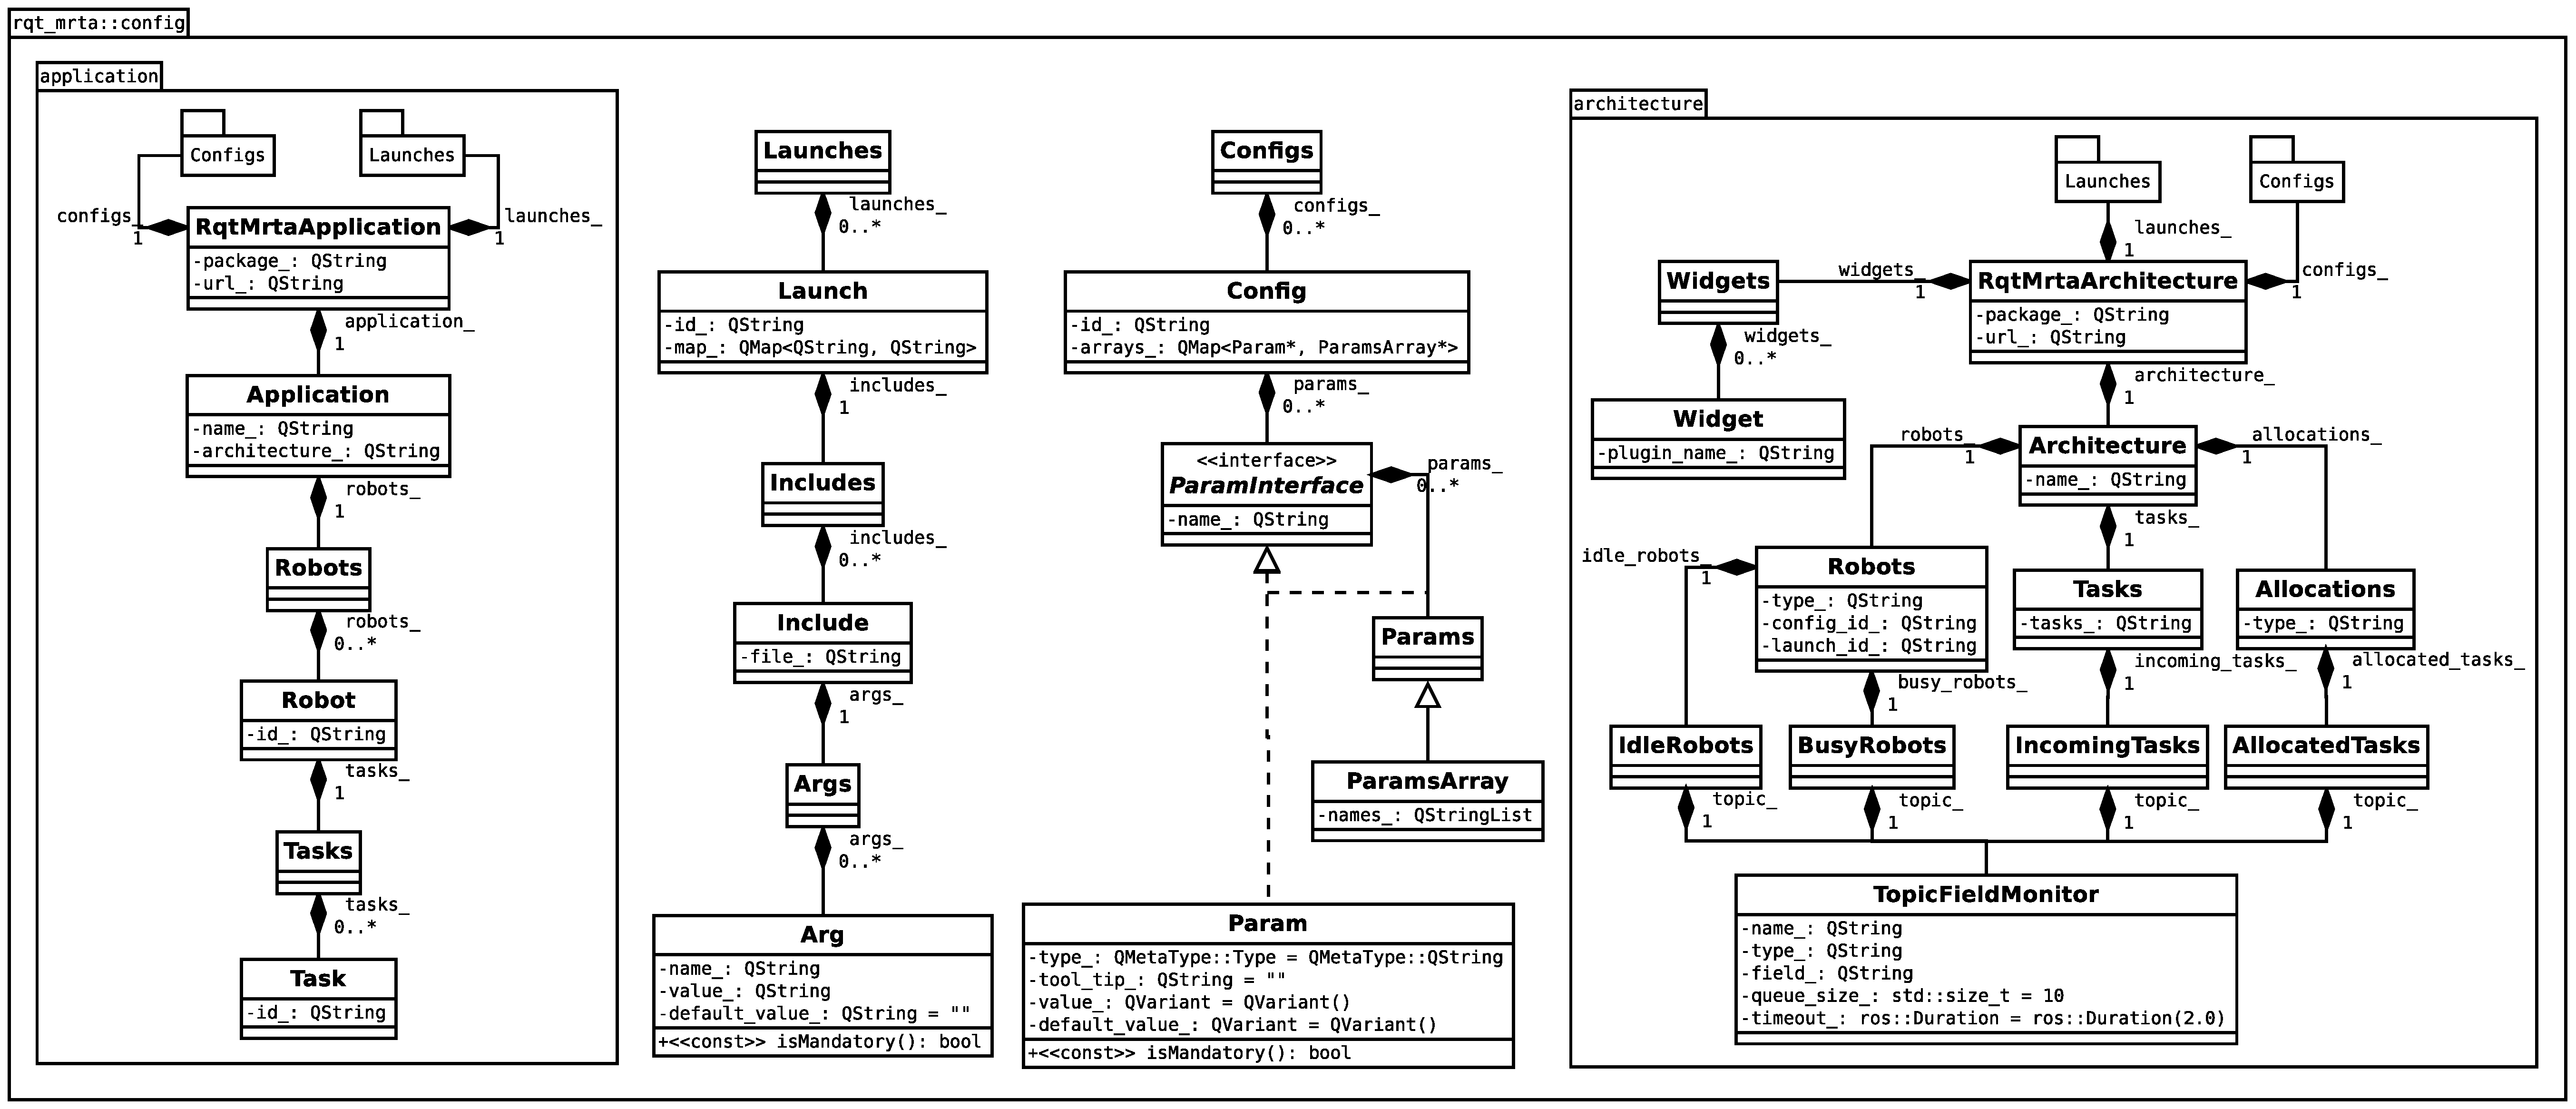
\includegraphics[width=.97\textheight,angle=90]{Figuras/3_desenvolvimento/rqt_mrta_model_uml.eps}
            \caption{Diagrama de classes da camada do modelo.} \label{fig:rqt_mrta_model_uml}
        \end{figure}
        
        Cada classe mostrada na Figura \ref{fig:rqt_mrta_model_uml} representa uma \textit{tag} não-folha. E as \textit{tags} folhas são membros de alguma classe do modelo. Alguma dessas classes possuem métodos utilitários que ajudam na geração de arquivos. São elas:
        
        \begin{itemize}
            \item \textit{RqtMrtaArchitecture}: possui métodos que facilitam a leitura e escrita de arquivos de configuração de arquitetura;
            
            \item \textit{RqtMrtaApplication}: possui métodos que facilitam a leitura e escrita de arquivos de configuração de aplicação;
            
            \item \textit{Launches}: possui método que auxiliam na chamada pela geração e organização dos arquivos de inicialização de uma configuração de aplicação;
            
            \item \textit{Launch}: possui um método que facilita a escrita de arquivos de inicialização (na extensão \textit{.launch});
            
            \item \textit{Configs}: possui métodos que auxiliam na chamada pela geração e organização dos arquivos de parâmetros de uma configuração de aplicação;
            
            \item \textit{Config}: possui um método que facilita a escrita de arquivos de parâmetros (na extensão \textit{.yaml}).
        \end{itemize}
        
    \section{Camada de visualização} \label{subsec:rqt_mrta_view}
        O Qt \cite{ref:yafei2012qt} possui uma ferramenta chamada \textit{Qt Designer} que permitiu o desenvolvimento da camada de apresentação (\textit{view}) deste projeto, pois ela representa graficamente a disposição dos componentes Qt para a customização de janelas (\textit{widgets}, \textit{dialogs} e \textit{wizards}). A partir dessas representações foram gerados arquivos de extensão UI (\textit{User Interface}) que armazenam a árvore de relação entre os componentes Qt e formata os dados em XML. Finalmente, em tempo de compilação, os arquivos UI foram convertidos para classes codificadas em C++.
        
        \subsection{\textit{Widget} principal do \textit{rqt\_mrta}} \label{subsec:rqt_mrta_front}
            A Figura \ref{fig:rqt_mrta_front} mostra o \textit{widget} principal do \textit{plugin rqt\_mrta}. No parte superior da janela se localiza a barra de ferramentas, a qual possui os botões com as seguintes função:
            
            \begin{itemize}
                \item \textbf{Nova aplicação}: abre um novo \textit{wizard} para a criação de uma nova aplicação. Se este \textit{wizard} é finalizado com sucesso, o \textit{widget} principal do \textit{plugin} se adapta conforme as configurações da nova aplicação criada;
                
                \item \textbf{Carregar aplicação}: abre um \textit{dialog} para a seleção de uma aplicação já criada anteriormente. Se uma das aplicações listadas é selecionada, então o \textit{widget} principal do \textit{plugin} se adapta conforme as configurações desta aplicação;
                
                \item \textbf{Executar aplicação}: executa os arquivos de inicialização da aplicação carregada. Esta função não está habilitada ainda;
                
                \item \textbf{Nova arquitetura}: abre um novo \textit{wizard} para a configuração e cadastro de uma nova arquitetura. Se este \textit{wizard} é finalizado com sucesso, o \textit{widget} principal do \textit{plugin} se adapta conforme as configurações da nova arquitetura cadastrada. Esta função não está habilitada ainda;
                
                \item \textbf{Carregar arquitetura}: abre um \textit{dialog} para a seleção de uma arquitetura já cadastrada. Se uma das arquiteturas listadas é selecionada, então o \textit{widget} principal do \textit{plugin} se adapta conforme as configurações desta arquitetura, isto é, serão carregados os \textit{widgets} fornecidos pela arquitetura.
            \end{itemize}
        
            \begin{figure}[htb]
                \centering
                \includegraphics[width=.8\textwidth]{Figuras/3_desenvolvimento/rqt_mrta_front.png}
                \caption{Janela principal do \textit{plugin rqt\_mrta}.} \label{fig:rqt_mrta_front}
            \end{figure}
            
            A parte central da janela mostra dois painéis, o painel da esquerda mostra o estado de cada robô do sistema e o painel da direita mostra o estado das tarefas do sistema.
        
        \subsection{\textit{Wizard} para criação de nova aplicação} \label{subsec:wizard_new_app}
            A Figura \ref{fig:example_new_app} mostra as telas do \textit{wizard} para a criação de uma nova aplicação, onde são definidos seus os dados gerais, é selecionado uma das arquiteturas registradas, são definidos os robôs do sistema, bem como, as tarefas que cada um é capaz de realizar. Em seguida, cada arquivo necessário para parametrizar a arquitetura escolhida é preenchido e, finalmente, é mostrado quais arquivos e pastas serão criados a partir das informações dadas. 
            
            Ao final deste procedimento, será criado um pacote contendo o arquivos manifesto (configurado conforme \ref{subsec:app_config_rgst}), CMakeLists.txt e de configuração de aplicação. Em seguida, são gerados os arquivos de parâmetro e de inicialização a partir dos dados inseridos pelo usuário. Os arquivos de parâmetro serão agrupados na pasta \textit{config} do pacote gerado e os arquivos de inicialização serão agrupados na pasta \textit{launch} do pacote gerado.
            
            \begin{figure}[htb]
                \centering
                \subfloat[Dados gerais da aplicação.]{
                    \includegraphics[width=.31\textwidth]{Figuras/3_desenvolvimento/example_def_app.png}
                    \label{fig:example_def_app}
                }
                \subfloat[Escolha da arquitetura.]{
                    \includegraphics[width=.31\textwidth]{Figuras/3_desenvolvimento/example_def_arch.png}
                    \label{fig:example_def_arch}
                }
                \subfloat[Definição dos robôs do sistema.]{
                    \includegraphics[width=.31\textwidth]{Figuras/3_desenvolvimento/example_def_robots.png}
                    \label{fig:example_def_robots}
                }
                
                \subfloat[Parametrização da arquitetura.]{
                    \includegraphics[width=.31\textwidth]{Figuras/3_desenvolvimento/example_def_params.png}
                    \label{fig:example_def_params}
                }
                \subfloat[Sumário.]{
                    \includegraphics[width=.31\textwidth]{Figuras/3_desenvolvimento/example_summary.png}
                    \label{fig:example_summary}
                }
                \caption{\textit{Wizard} para a criação de uma nova aplicação.} \label{fig:example_new_app}
            \end{figure}
            
            A primeira tela do \textit{wizard} de novas aplicações, mostrado na Figura \ref{fig:example_def_app}, coleta os dados gerais da aplicação. Estes dados serão utilizados na geração do arquivo manifesto do pacote. Caso o \textit{workspace} dado não seja um \textit{workspace} do ROS, o usuário é alertado de que será criado um novo \textit{workspace} no diretório especificado. Deve-se atentar para o preenchimento correto do endereço eletrônico do mantenedor do pacote. Caso contrário, o pacote não poderá ser compilado. Após o preenchimento de todos os dados obrigatórios, o usuário pode prosseguir para a próxima tela.
            
            Em seguida, pede-se para o usuário escolher uma arquitetura, conforme Figura \ref{fig:example_def_arch}. A escolha pode ser realizada com o auxílio de três filtros: pelo tipo dos robôs (ST \textit{versus} MT), pelo tipo das tarefas (SR \textit{versus} MR) e pelo tipo das alocações (IA \textit{versus} TA), conforme a taxonomia revisada na Seção \ref{subsec:taxonomia_mrta}. Assim que o usuário passa para a próxima tela, o \textit{rqt\_mrta} carrega o arquivo de configuração da arquitetura selecionada. Logo, os \textit{templates} dos arquivos de parâmetros e de inicialização estarão disponíveis na memória para a geração dos arquivos necessários para a aplicação.
            
            Após a seleção da arquitetura, pede-se para identificar os robôs do sistema. A interface para a entrada desses dados é mostrada na Figura \ref{fig:example_def_robots}. A partir dos robôs e dos \textit{templates} de arquivos de parâmetros do arquivo de configuração de arquitetura carregado, pede-se para o usuário preencher os arquivos de parâmetros para cada robô e os demais arquivos que não são associados diretamente aos robôs, conforme mostra a Figura \ref{fig:example_def_params}.
            
            Os campos que aparecem o símbolo asterisco (*), identificam para o usuário quais entradas devem ser preenchidas obrigatoriamente. O usuário fica impossibilitado de avançar para a próxima tela enquanto ele não tenha preenchido todas entradas obrigatórias. Isso garante que ao final do procedimento, a arquitetura estará devidamente configurada e será possível gerar o pacote da aplicação com sucesso.
            
            Na última tela do \textit{wizard}, após o preenchimento de todos parâmetros obrigatórios, o usuário pode ver um resume das ações que serão realizadas pelo \textit{plugin} ao concluir o procedimento. Conforme mostra a Figura \ref{fig:example_summary}, esta tela informa se o \textit{plugin} iniciará um novo \textit{workspace} do ROS (conforme necessidade), mostra o diretório em que o pacote da aplicação será criado, bem como, os arquivos e pastas que serão gerados neste pacote.
            
            \begin{figure}[htb]
                \centering
                \subfloat[Pacote.]{
                    \includegraphics[width=.4\textwidth]{Figuras/3_desenvolvimento/example_pkg.png}
                    \label{fig:example_pkg}
                }
                \subfloat[Arquivos de parâmetro.]{
                    \includegraphics[width=.4\textwidth]{Figuras/3_desenvolvimento/example_pkg_config.png}
                    \label{fig:example_pkg_config}
                }
                
                \subfloat[Arquivos de inicialização.]{
                    \includegraphics[width=.4\textwidth]{Figuras/3_desenvolvimento/example_pkg_launch.png}
                    \label{fig:example_pkg_launch}
                }
                \caption{Pastas e arquivos gerados após a criação de uma aplicação.} \label{fig:example}
            \end{figure}
            
        \subsection{\textit{Dialogs} para a seleção de arquiteturas e aplicações} \label{subsec:dialogs_open}
            As Figuras \ref{fig:opening_arch} e \ref{fig:opening_app} mostram, respectivamente, as janelas para a seleção de uma arquitetura e de uma aplicação para o carregamento do seu arquivo de configuração. Ao invés dos usuários navegarem pelos diretórios do sistema operacional procurando o arquivo desejado, são listados para ele os pacotes que foram devidamente configurados, conforme descrito nas Seções \ref{sec:arch_config} e \ref{sec:app_config}, respectivamente. 
            
            \begin{figure}[htb]
                \centering
                \subfloat[de uma arquitetura.]{
                    \includegraphics[height=.11\textheight]{Figuras/3_desenvolvimento/opening_arch.png}
                    \label{fig:opening_arch}
                }
                \subfloat[de uma aplicação.]{
                    \includegraphics[height=.11\textheight]{Figuras/3_desenvolvimento/opening_app.png}
                    \label{fig:opening_app}
                }
                \caption{Carregando um arquivo de configuração} \label{fig:opening_config}
            \end{figure}
        
    \section{Camada de controle} \label{subset:rqt_mrta_controller}
        A camada de controle auxilia na supervisão do sistema em tempo de execução. Esta camada encapsula classes que monitoram os tópicos do ROS para a verificação de alteração do estado dos robôs, tarefas e alocações do sistema. Deste modo, a camada de visualização só se preocupa em exibir graficamente os estados dessas entidades no \textit{widget} principal do \textit{rqt\_mrta}.
        
        A Figura \ref{fig:rqt_mrta_controller_uml} mostra o diagrama UML (\textit{Unified Modeling Language}) que relaciona as classes do modelo utilizado na camada de controle do \textit{rqt\_mrta}. Será detalhada a seguir cada classe contida neste diagrama.
        
        \begin{figure}[p]
            \centering
            \includegraphics[height=\textwidth,angle=90]{Figuras/3_desenvolvimento/rqt_mrta_controller_uml.eps}
            \caption{Diagrama de classes do camada de controle.} \label{fig:rqt_mrta_controller_uml}
        \end{figure}
        
        As classes principais deste modelo são: \textit{System}, \textit{Problem}, \textit{Robot}, \textit{Task}, \textit{Allocation} e \textit{Architecture}, cuja relação se dá mediante a definição de um problema de atribuição de tarefa em sistema multirrobô. Logo, como o sistema possui vários robôs e um problema de alocação de tarefa para ser resolvido, um objeto do tipo \textit{System} é composto por vários objetos do tipo \textit{Robot} e também de uma instância de objeto da classe \textit{Problem}. A classe \textit{Problem} tem como responsabilidade relacionar cada tarefa a ser executada com um robô (caso o tipo das tarefas do sistema seja SR) ou um grupo de robôs (caso o tipo das tarefas do sistema sejam MR) através de uma alocação. Logo, um objeto do tipo \textit{Problem} é composto por vários objetos do tipo \textit{Task}, vários do tipo \textit{Allocation} e uma instância de \textit{Architecture}. A classe \textit{Architecture} apenas armazena a classe de problema que pode ser resolvido pela arquitetura MRTA escolhida. 
        
        As classes \textit{Robot}, \textit{Task} e \textit{Allocation} são muito parecidas. Elas mantêm uma identificação única para cada robô, tarefa e alocação identificados no sistema, respectivamente. Contudo, objetos da classe \textit{Allocation} têm uma instância de \textit{Task} e pode ter um ou vários objetos \textit{Robot}, dependendo do tipo das tarefas que a arquitetura MRTA escolhida resolve. Cada uma dessas três classes ainda possuem um objeto do tipo \textit{History} que armazena \textit{logs} das alterações de estado, o qual é monitorado pelo objeto \textit{StateMonitor} que elas possuem. Objetos \textit{StateMonitor}, por sua vez, são compostos por vários objetos \textit{SampleHolder}, um para cada estado sendo monitorado. Esta classe funciona como se fosse um demultiplexador, direcionando o evento na sua entrada para a saída apropriada. Isto é, se o objeto \textit{StateMonitor} de um dado robô recebe a informação que ele se encontra no estado \textit{Busy} (ocupado), esse encaminha esta informação para o objeto \textit{SampleHolder} que mantém o histórico de notificações desse estado. Portanto, a classe \textit{SampleHolder} é responsável por identificar as rampas de subida e de descida de um dado estado do objeto em monitoramento. Este objeto leva em consideração um parâmetro (\textit{timeout}) que especifica o tempo máximo considerado para manter o dado estado em nível lógico alto.
        
        Voltando a classe \textit{System}, objetos desse tipo ainda são compostos por vários objetos do tipo \textit{Monitor} que pode ser especificado para os tipos \textit{RobotMonitor}, \textit{TaskMonitor} e \textit{AllocationMonitor}. Cada um tem a função de monitorar um campo específico de uma dada mensagem provida de um tópico específico, conforme os parâmetros do arquivo de configuração da arquitetura MRTA escolhida.  Como objeto \textit{Monitor} analisa um estado específico de um conjunto de entidades da mesma natureza. Por exemplo, objetos \textit{RobotMonitor} analisam um dado estado dos robôs do sistema; objetos do tipo \textit{TaskMonitor} analisam um estado específico para as tarefas do sistema; e, por fim, um estado específico das alocações do sistema é analisado em objetos do tipo \textit{AllocationMonitor}. Assim, de forma semelhante à classe \textit{StateMonitor}, as classes do tipo \textit{Monitor} têm um papel similar a um demultiplexador, entregando a notificação recebida ao objeto \textit{StateMonitor} apropriado. Exemplificando, seja um objeto \textit{RobotMonitor} que observa o tópico \textit{/busy\_robots} onde os robôs do sistema publicam quais atividades eles estão desempenhando. Ao ser notificado da chegada de uma mensagem cujo o remetente é o robô \textit{robot1}, este monitor encaminhará uma notificação para o objeto \textit{StateMonitor} do \textit{robot1} dizendo que ele se encontra no estado \textit{Busy}. Por sua vez, o objeto \textit{StateMonitor} de \textit{robot1} direciona está notificação para o \textit{SampleHolder} que mantém o histórico do estado \textit{Busy} de \textit{robot1}. Finalmente, a cada rampa de subida ou descida de um dos seus estados, \textit{robot1} atualiza seu estado atual.
        
        Perceba que a classe \textit{Monitor} faz uso de duas classes utilitárias:
        
        \begin{itemize}
            \item \textit{utilities::MessageSubscriberRegistry}: faz uso da biblioteca \textit{variant\_topic\_tools}\footnote{\url{https://github.com/ethz-asl/variant}} para a subscrição em tópicos cujo tipo é desconhecido em tempo de compilação.  Através do mecanismo \textit{signal}\footnote{Um \textit{signal} é emitido quando um evento particular ocorre em um \textit{QObject}.} - \textit{slot}\footnote{Um \textit{slot} é uma função de um \textit{QObject} que é chamada em resposta a um \textit{signal} específico.} do Qt \cite{ref:yafei2012qt}, sempre quando uma nova mensagem é recebida, essa classe notifica todas as outras que têm interesse no recebimento de mensagens de um dado tópico;
            
            \item \textit{utilities::MessageFieldSubscriber}: utiliza a classe \textit{utilities::MessageSubscriberRegistry} para a notificação do recebimento de mensagens de um tópico particular. Ao ser notificado, essa classe avalia se o valor do campo especificado confere com o valor desejado. Sempre que esta condição é satisfeita, é emitido um \textit{signal} deste evento para as classes interessadas.
        \end{itemize}
         
        O uso dessas classes utilitárias pelo \textit{Monitor} garante flexibilidade no cadastro das arquiteturas, pois não é necessário fazer adaptações para que a arquitetura se adéque a um suposto padrão estipulado pelo \textit{rqt\_mrta}.
    
\chapter[Experimentos e Resultados]{Experimentos e Resultados} \label{cap:resultados}

\chapter[Conclusão e Trabalhos Futuros]{Conclusão e Trabalhos Futuros} \label{cap:conclusao}

    \section{Conclusão}
        Este trabalho apresentou o desenvolvimento de uma interface gráfica de usuário integrada com o \textit{framework} ROS com o intuito de facilitar a parametrização de arquiteturas de alocação de tarefa em aplicações com múltiplos robôs. A interface desenvolvida fornece serviços de criação e supervisão de aplicações multirrobô no ROS. Durante o processo de criação de aplicação é solicitado o preenchimento correto dos parâmetros da arquitetura selecionada. 
        
        Primeiramente, este trabalho apresentou um estudo sobre sistemas multirrobô, identificando suas vantagens perante um sistema de um único robô, bem como, suas características. Em seguida, foi revisado o problema de alocação de tarefa nesses sistemas e como eles podem ser classificados. Verificou-se a existência de várias arquiteturas que visam resolver estes problemas. Uma análise do ROS foi feita apresentando os seus conceitos básicos e o desenvolvimento de interfaces gráficas de usuário integrada com o \textit{framework}. Por fim, pesquisas relacionadas ao desenvolvimento de arquiteturas MRTA mostraram que existem poucas aproximações genéricas implementadas no ROS e que normalmente elas não possuem boa documentação.
        
        O capítulo de desenvolvimento mostrou como são estruturados os arquivos de configuração de arquitetura e de  aplicação. Em cada caso, foi apresentado o processo de cadastro de arquiteturas e aplicações de modo que o pacote \textit{rqt\_mrta} identificá-las. Posteriormente, foram explicadas as camadas de modelo, visualização e controle do projeto \textit{rqt\_mrta}. 
    
        Uma implementação genérica da arquitetura ALLIANCE foi desenvolvida no pacote \textit{alliance} para o teste do pacote \textit{rqt\_mrta}. Para que esta arquitetura pudesse ser utilizada por aplicações multirrobô, foi criado o arquivo de configuração da arquitetura do \textit{alliance}, exportando a localização deste arquivo através do seu manifesto. Em seguida, verificou-se que o cadastro desta arquitetura foi realizado com sucesso.
        
        Uma aplicação com vários robôs em um sistema de patrulhamento foi criada e simulada em conjunto com o pacote \textit{alliance} para validar as funcionalidades do \textit{plugin rqt\_mrta}. Durante a sua criação (via \textit{wizard}) foram inseridos os dados gerais da aplicação, selecionada a arquitetura do pacote \textit{alliance}, indicados os robôs do sistema e, por fim, preenchidos os parâmetros obrigatórios da arquitetura selecionada. Ao final deste procedimento, foi iniciado um novo \textit{workspace} do ROS onde foi criado um novo pacote ROS contendo os arquivos gerados a partir do preenchimento dos dados da aplicação. Na sequência, os arquivos gerados foram examinados e utilizados na inicialização dos nós necessários para a execução da arquitetura selecionada. Foi averiguado que a comunicação entre os nós da arquitetura estava correta.
        
        Com o auxilio de um simulador, a aplicação foi executada juntamente com os nós da arquitetura do pacote \textit{alliance}. Durante sua execução, os recursos de supervisão gráfica do \textit{plugin rqt\_mrta} foi analisado.
        
        Concluindo, o processo de criação de aplicação multirrobô através do \textit{rqt\_mrta} mostrou que, após a configuração e cadastro da arquitetura, sua parametrização para o uso em aplicações torna-se mais intuitiva devido a existência de uma documentação mínima. %Além disso, o \textit{plugin} facilita a criação dos arquivos exigidos pela arquitetura.
        
    \section{Trabalhos Futuros}
        Uma melhoria significativa desta aplicação seria possibilitar a inscrição de novas arquiteturas devidamente configuradas no repositório deste projeto. De modo que, sempre que uma nova inscrição ocorresse no \textit{rqt\_mrta}, seria solicitada uma nova atualização a todos usuários do pacote \textit{rqt\_mrta} para baixar e instalar a nova arquitetura inscrita. Isso eliminaria a necessidade de procurar novas abordagens de arquitetura por seus usuários e ajudaria o desenvolvedor de arquiteturas a impulsionar seu projeto na comunidade ROS.
        
        Enfim, a adição de mais alguns recurso no \textit{plugin} resultaria em um maior envolvimento do desenvolvedores e usuários de arquiteturas, como:
        
        \begin{itemize}
            \item a comparação do uso de arquiteturas diferentes em uma mesma aplicação para a análise de desempenho;
            
            \item geração de relatórios gráficos e numéricos durante a execução da aplicação;
            
            \item inicialização e parada da aplicação através do \textit{plugin};
            
            \item serviços de agendamento;
            
            \item simulação de tarefas para validação da arquitetura em desenvolvimento;
            
            \item entre outros.
        \end{itemize}
        
        

% Elementos pós-textuais
\postextual
% Apêndices - opcional
\apendices
\partapendices 	% imprime uma página indicando o início dos apêndices
\chapter{Funções Temporais} \label{app:funcoes}

    \section{Funções Degraus} \label{sec:funcoes_degraus}
    
        A Figura \ref{fig:funcoes_degraus} mostra duas funções degraus: ascendente \ref{fig:funcao_degrau_ascendente} e descendente \ref{fig:funcao_degrau_descendente}.
    
        \begin{figure}[htb]
            \centering
            \subfloat[Função degrau ascendente.]{
                \resizebox{0.45\textwidth}{!}{\input{Figuras/apendice_a/ascending_step_function}}
                \label{fig:funcao_degrau_ascendente}
            }
            \subfloat[Função degrau descendente.]{
                \resizebox{0.45\textwidth}{!}{\input{Figuras/apendice_a/decending_step_function}}
                \label{fig:funcao_degrau_descendente}
            }
            \caption{Funções degraus.} \label{fig:funcoes_degraus}
        \end{figure}
        
        \begin{equation} \label{eq:funcao_degrau_ascendente}
            q(t) =
            \begin{cases}
                q_0 ,& t \leq t_0 \\
                q_f ,& t > t_0
            \end{cases}
        \end{equation}
        
        \begin{equation} \label{eq:funcao_degrau_descendente}
            q(t) =
            \begin{cases}
                q_f ,& t \leq t_0 \\
                q_0 ,& t > t_0
            \end{cases}
        \end{equation}
    
    \section{Funções Pulsos} \label{sec:funcoes_pulsos}
    
        A Figura \ref{fig:funcoes_pulsos} mostra duas funções pulsos: ascendente \ref{fig:funcao_pulso_ascendente} e descendente \ref{fig:funcao_pulso_descendente}.
    
        \begin{figure}[htb]
            \centering
            \subfloat[Função pulso ascendente.]{
                \resizebox{0.45\textwidth}{!}{\input{Figuras/apendice_a/ascending_pulse_function}}
                \label{fig:funcao_pulso_ascendente}
            }
            \subfloat[Função degrau descendente.]{
                \resizebox{0.45\textwidth}{!}{\input{Figuras/apendice_a/decending_pulse_function}}
                \label{fig:funcao_pulso_descendente}
            }
            \caption{Funções pulsos.} \label{fig:funcoes_pulsos}
        \end{figure}
        
        \begin{equation} \label{eq:funcao_pulso_ascendente}
            q(t) =
            \begin{cases}
                q_0 ,& t \leq t_0 \\
                q_f ,& t > t_0
            \end{cases}
        \end{equation}
        
        \begin{equation} \label{eq:funcao_pulso_descendente}
            f(t) =
            \begin{cases}
                q_f ,& t \leq t_0 \\
                q_0 ,& t > t_0
            \end{cases}
        \end{equation}
    
    \section{Funções Lineares} \label{sec:funcoes_lineares}
    
        A Figura \ref{fig:funcoes_lineares} mostra duas funções lineares: ascendente \ref{fig:funcao_linear_ascendente} e descendente \ref{fig:funcao_linear_descendente}.
    
        \begin{figure}[htb]
            \centering
            \subfloat[Função linear ascendente.]{
                \resizebox{0.45\textwidth}{!}{% Graphic for TeX using PGF
% Title: ../figures/functions/ascending_linear_function.dia
% Creator: Dia v0.97.2
% CreationDate: Sun Oct 15 13:33:43 2017
% For: adrianohrl
% \usepackage{tikz}
% The following commands are not supported in PSTricks at present
% We define them conditionally, so when they are implemented,
% this pgf file will use them.
\ifx\du\undefined
  \newlength{\du}
\fi
\setlength{\du}{15\unitlength}
\begin{tikzpicture}
\pgftransformxscale{1.000000}
\pgftransformyscale{-1.000000}
\definecolor{dialinecolor}{rgb}{0.000000, 0.000000, 0.000000}
\pgfsetstrokecolor{dialinecolor}
\definecolor{dialinecolor}{rgb}{1.000000, 1.000000, 1.000000}
\pgfsetfillcolor{dialinecolor}
% setfont left to latex
\definecolor{dialinecolor}{rgb}{0.000000, 0.000000, 0.000000}
\pgfsetstrokecolor{dialinecolor}
\node at (34.500000\du,21.221250\du){$t_f$};
\pgfsetlinewidth{0.050000\du}
\pgfsetdash{{1.000000\du}{1.000000\du}}{0\du}
\pgfsetdash{{0.250000\du}{0.250000\du}}{0\du}
\pgfsetbuttcap
{
\definecolor{dialinecolor}{rgb}{0.000000, 0.000000, 0.000000}
\pgfsetfillcolor{dialinecolor}
% was here!!!
\definecolor{dialinecolor}{rgb}{0.000000, 0.000000, 0.000000}
\pgfsetstrokecolor{dialinecolor}
\draw (34.500000\du,20.000000\du)--(34.500000\du,12.500000\du);
}
% setfont left to latex
\definecolor{dialinecolor}{rgb}{0.000000, 0.000000, 0.000000}
\pgfsetstrokecolor{dialinecolor}
\node at (23.000000\du,13.721250\du){$q_f$};
\pgfsetlinewidth{0.050000\du}
\pgfsetdash{{0.250000\du}{0.250000\du}}{0\du}
\pgfsetdash{{0.250000\du}{0.250000\du}}{0\du}
\pgfsetbuttcap
{
\definecolor{dialinecolor}{rgb}{0.000000, 0.000000, 0.000000}
\pgfsetfillcolor{dialinecolor}
% was here!!!
\definecolor{dialinecolor}{rgb}{0.000000, 0.000000, 0.000000}
\pgfsetstrokecolor{dialinecolor}
\draw (24.000000\du,13.500000\du)--(36.500000\du,13.500000\du);
}
% setfont left to latex
\definecolor{dialinecolor}{rgb}{0.000000, 0.000000, 0.000000}
\pgfsetstrokecolor{dialinecolor}
\node at (26.000000\du,21.221250\du){$t_0$};
\pgfsetlinewidth{0.050000\du}
\pgfsetdash{{0.250000\du}{0.250000\du}}{0\du}
\pgfsetdash{{0.250000\du}{0.250000\du}}{0\du}
\pgfsetbuttcap
{
\definecolor{dialinecolor}{rgb}{0.000000, 0.000000, 0.000000}
\pgfsetfillcolor{dialinecolor}
% was here!!!
\definecolor{dialinecolor}{rgb}{0.000000, 0.000000, 0.000000}
\pgfsetstrokecolor{dialinecolor}
\draw (26.000000\du,12.500000\du)--(26.000000\du,20.000000\du);
}
% setfont left to latex
\definecolor{dialinecolor}{rgb}{0.000000, 0.000000, 0.000000}
\pgfsetstrokecolor{dialinecolor}
\node at (23.000000\du,19.221250\du){$q_0$};
\pgfsetlinewidth{0.050000\du}
\pgfsetdash{{0.250000\du}{0.250000\du}}{0\du}
\pgfsetdash{{0.250000\du}{0.250000\du}}{0\du}
\pgfsetbuttcap
{
\definecolor{dialinecolor}{rgb}{0.000000, 0.000000, 0.000000}
\pgfsetfillcolor{dialinecolor}
% was here!!!
\definecolor{dialinecolor}{rgb}{0.000000, 0.000000, 0.000000}
\pgfsetstrokecolor{dialinecolor}
\draw (24.000000\du,19.000000\du)--(36.500000\du,19.000000\du);
}
\pgfsetlinewidth{0.150000\du}
\pgfsetdash{}{0pt}
\pgfsetdash{}{0pt}
\pgfsetbuttcap
{
\definecolor{dialinecolor}{rgb}{0.000000, 0.000000, 0.000000}
\pgfsetfillcolor{dialinecolor}
% was here!!!
\definecolor{dialinecolor}{rgb}{0.000000, 0.000000, 0.000000}
\pgfsetstrokecolor{dialinecolor}
\draw (23.960000\du,19.000000\du)--(26.070000\du,19.000000\du);
}
\pgfsetlinewidth{0.150000\du}
\pgfsetdash{}{0pt}
\pgfsetdash{}{0pt}
\pgfsetbuttcap
{
\definecolor{dialinecolor}{rgb}{0.000000, 0.000000, 0.000000}
\pgfsetfillcolor{dialinecolor}
% was here!!!
\definecolor{dialinecolor}{rgb}{0.000000, 0.000000, 0.000000}
\pgfsetstrokecolor{dialinecolor}
\draw (34.430000\du,13.500000\du)--(36.570000\du,13.500000\du);
}
\pgfsetlinewidth{0.150000\du}
\pgfsetdash{}{0pt}
\pgfsetdash{}{0pt}
\pgfsetbuttcap
{
\definecolor{dialinecolor}{rgb}{0.000000, 0.000000, 0.000000}
\pgfsetfillcolor{dialinecolor}
% was here!!!
\definecolor{dialinecolor}{rgb}{0.000000, 0.000000, 0.000000}
\pgfsetstrokecolor{dialinecolor}
\draw (25.941230\du,19.038028\du)--(34.558770\du,13.461972\du);
}
\pgfsetlinewidth{0.100000\du}
\pgfsetdash{}{0pt}
\pgfsetdash{}{0pt}
\pgfsetbuttcap
{
\definecolor{dialinecolor}{rgb}{0.000000, 0.000000, 0.000000}
\pgfsetfillcolor{dialinecolor}
% was here!!!
\pgfsetarrowsend{stealth}
\definecolor{dialinecolor}{rgb}{0.000000, 0.000000, 0.000000}
\pgfsetstrokecolor{dialinecolor}
\draw (23.000000\du,20.000000\du)--(37.000000\du,20.000000\du);
}
% setfont left to latex
\definecolor{dialinecolor}{rgb}{0.000000, 0.000000, 0.000000}
\pgfsetstrokecolor{dialinecolor}
\node at (38.000000\du,20.221250\du){$t$};
\pgfsetlinewidth{0.100000\du}
\pgfsetdash{}{0pt}
\pgfsetdash{}{0pt}
\pgfsetbuttcap
{
\definecolor{dialinecolor}{rgb}{0.000000, 0.000000, 0.000000}
\pgfsetfillcolor{dialinecolor}
% was here!!!
\pgfsetarrowsend{stealth}
\definecolor{dialinecolor}{rgb}{0.000000, 0.000000, 0.000000}
\pgfsetstrokecolor{dialinecolor}
\draw (24.000000\du,21.000000\du)--(24.000000\du,12.000000\du);
}
% setfont left to latex
\definecolor{dialinecolor}{rgb}{0.000000, 0.000000, 0.000000}
\pgfsetstrokecolor{dialinecolor}
\node at (24.000000\du,11.221250\du){$q(t)$};
\end{tikzpicture}
}
                \label{fig:funcao_linear_ascendente}
            }
            \subfloat[Função linear descendente.]{
                \resizebox{0.45\textwidth}{!}{\input{Figuras/apendice_a/decending_linear_function}}
                \label{fig:funcao_linear_descendente}
            }
            \caption{Funções lineares.} \label{fig:funcoes_lineares}
        \end{figure}
        
        \begin{equation} \label{eq:funcao_linear_ascendente}
            q(t) =
            \begin{cases}
                q_0 ,& t \leq t_0 \\
                (q_f - q_0)\dfrac{t - t_0}{t_f - t_0} + q_0 ,& t_0 < t \leq t_f \\
                q_f ,& t > t_f
            \end{cases}
        \end{equation}
        
        \begin{equation} \label{eq:funcao_linear_descendente}
            q(t) =
            \begin{cases}
                q_f & t \leq t_0 \\
                (q_0 - q_f)\dfrac{t - t_0}{t_f - t_0} + q_f ,& t_0 < t \leq t_f \\
                q_0 & t > t_f
            \end{cases}
        \end{equation}
    
    \section{Função Exponenciais} \label{sec:funcoes_exponenciais}
    
        A Figura \ref{fig:funcoes_exponenciais} mostra duas funções exponenciais: ascendente \ref{fig:funcao_exponencial_ascendente} e descendente \ref{fig:funcao_exponencial_descendente}.
    
        \begin{figure}[htb]
            \centering
            \subfloat[Função exponencial ascendente.]{
                \resizebox{0.45\textwidth}{!}{\input{Figuras/apendice_a/ascending_exponential_function}}
                \label{fig:funcao_exponencial_ascendente}
            }
            \subfloat[Função exponencial descendente.]{
                \resizebox{0.45\textwidth}{!}{\input{Figuras/apendice_a/decending_exponential_function}}
                \label{fig:funcao_exponencial_descendente}
            }
            \caption{Funções exponenciais.} \label{fig:funcoes_exponenciais}
        \end{figure}
        
        \begin{equation} \label{eq:funcao_exponencial_ascendente}
            q(t) =
            \begin{cases}
                q_0 & t \leq t_0 \\
                q_f - (q_f - q_0) e^{-K\dfrac{t - t_0}{t_f - t_0}} ,& t_0 < t \leq t_f \\
                q_f & t > t_f
            \end{cases}
        \end{equation}
        
        \begin{equation} \label{eq:funcao_exponencial_descendente}
            q(t) =
            \begin{cases}
                q_f & t \leq t_0 \\
                q_0 - (q_0 - q_f) e^{-K\dfrac{t - t_0}{t_f - t_0}} ,& t_0 < t \leq t_f \\
                q_0 & t > t_f
            \end{cases}
        \end{equation}
% Anexos - opcional
\anexos
\partanexos		% imprime uma página indicando o início dos anexos
\input{5_Anexos/anexo_a.tex}

\phantompart	% adiciona espaço no sumário
% Referências bibliográficas - obrigatório
\bibliography{6_Referencias/bibliografia.bib}
% Índice remissivo - opcional
\printindex	% imprime as páginas nas quais as macros \index{palavra a ser indexada} apareceram.

% Fim do documento
\end{document}